\documentclass[10pt,a4paper]{article}
\usepackage[margin=2.2cm]{geometry}
\usepackage{amsmath,amssymb,amsthm}
\usepackage{booktabs,array}
\usepackage{graphicx}
\usepackage{xcolor}
\usepackage{placeins}
\usepackage[colorlinks=true,linkcolor=blue!50!black,citecolor=blue!50!black,urlcolor=blue!50!black]{hyperref}
\usepackage{natbib}
\bibliographystyle{abbrvnat}
\setcitestyle{authoryear,round}

\newcommand{\vr}{\mathbf{r}}
\newcommand{\vn}{\hat{\mathbf{n}}}
\newcommand{\provisional}{\textcolor{orange!70!black}{\textsf{\small[provisional --- to be regenerated with Cavendish (S5)]}}}
% generated by scripts/realread.py
\newcommand{\SignalMax}{46}
\newcommand{\SignalMin}{43}
\newcommand{\SignalPlate}{4.4}
\newcommand{\LeadMax}{17}
\newcommand{\ClosedRel}{$3.0\times10^{-14}$}
\newcommand{\ClosedPhase}{$1.4\times10^{-12}$}
\newcommand{\WorstSampled}{$4.8\times10^{-2}$}
\newcommand{\WorstCentroid}{$5.1\times10^{-6}$}
\newcommand{\WorstSecond}{$2.0\times10^{-8}$}
\newcommand{\WorstSecondBody}{turned cube}
\newcommand{\WorstCentroidBody}{plate}
\newcommand{\AlignedSampled}{$4.8\times10^{-2}$}
\newcommand{\AlignedCentroid}{$4.9\times10^{-6}$}
\newcommand{\AlignedSecond}{$2.5\times10^{-10}$}
\newcommand{\GainCentroid}{$9.7\times10^{3}$}
\newcommand{\GainSecond}{$1.9\times10^{8}$}
\newcommand{\ArmClearance}{0.88}
\newcommand{\OrderZeroOneNear}{1.0--2.6}
\newcommand{\OrderZeroOneFar}{0.9--2.5}
\newcommand{\OrderSampledNear}{0.8--2.5}
\newcommand{\OrderSampledFar}{0.9--2.8}
\newcommand{\OrderFillNear}{2.0--4.4}
\newcommand{\OrderFillFar}{2.1--4.5}
\newcommand{\OrderCentroidNear}{2.8--4.1}
\newcommand{\OrderCentroidFar}{2.8--3.9}
\newcommand{\OrderSecondNear}{3.8--4.9}
\newcommand{\OrderSecondFar}{3.7--3.9}
\newcommand{\DecimDragon}{$3.4\times10^{-3}$}
\newcommand{\DecimArmadillo}{$3.3\times10^{-3}$}
\newcommand{\DecimBuddha}{$1.4\times10^{-3}$}
\newcommand{\SweepD}{$1.7\times10^{-11}$--$2.9\times10^{-10}$}
\newcommand{\SweepC}{$6.0\times10^{-9}$--$1.2\times10^{-7}$}
\newcommand{\SweepB}{$2.2\times10^{-5}$--$2.8\times10^{-3}$}

% The technique's name, in one place (the owner may choose another).
\newcommand{\cutcell}{cut-cell moments}
\newcommand{\Cutcell}{Cut-cell moments}

\title{Exact gravity of polyhedral boundary cells for simulating\\
atom-interferometer gravity gradiometers}
\author{Malachy Doherty\\
\small\textcolor{gray}{[affiliation --- placeholder, to be filled in by the author]}\\[4pt]
\small\textcolor{red!60!black}{\textbf{DRAFT for comments --- not submitted anywhere.}}\\
\small\textcolor{red!60!black}{Whether, where and with whom to publish is the author's decision.}}
\date{27 November 2026 (draft 3)}

\begin{document}
\maketitle

\begin{abstract}
A simulator of an atom-interferometer gravity gradiometer must turn every mass near the instrument
into a phase, and a voxelised world does so cell by cell. Where a body's surface crosses a cell,
the usual choices --- a cell full or empty, or a sampled fill fraction --- make an error of first
order in the pitch on faces aligned with the lattice, which for a tonne-scale body 1.5~m from an
AION-10 tower is $10^{-1}$~rad, three orders above the shot noise. We collect the closed form for
the potential and attraction of a uniform polyhedron (Werner \& Scheeres's face and edge form), derive
it, and give the rules that keep it accurate in double precision: the solid angle's numerator formed
as the face's height times twice its area, which keeps far-field rounding at $\varepsilon(R/s)^2$
rather than $\varepsilon(R/s)^3$, and the edge logarithm in a cancellation-free form near an edge.
Against a 40-digit evaluation our form loses $10^{-12}$ of $g$ at $R/s=100$, while an independent
line-integral implementation (ESA's) loses $10^{-9}$--$10^{-8}$. Storing instead each \emph{cut cell}'s mass, centroid and second moment
(\cutcell), computed exactly for the mesh, gives measured orders $3$ to $\geq 3.4$ in the pitch,
and a layered scheme --- clipped pieces near a tower, \cutcell{} in the middle, octree nodes
beyond ---
holds the representation error near $10^{-7}$~rad at 1.5~m with a 1/64~m pitch. On ten further
shapes --- an analytic sphere and torus, the Utah teapot, Suzanne, four Stanford scans, a cow and a CAD
part --- \cutcell{} reach $10^{-10}$--$10^{-9}$~rad at 1.5~m with 128 cells across a mesh, but two other
errors are larger: a mesh standing in for a curved shape is off by 0.03--2~rad (taking the cut
cells from the analytic surface removes it), and a decimated scan by $10^{-3}$~rad. On the sphere alone
adding the second moment makes the result worse, which we cannot yet explain. The chain from the
volume integral to faces and edges is formalised in Lean~4 with Mathlib: the edge integral, the
numerator identity, the divergence identities and the superposition of pieces are proven; the
divergence theorem for a general polyhedron is an explicit hypothesis, and for a rectangular box it
is Mathlib's theorem, so the box's face form carries no hypothesis at all.
\end{abstract}

\noindent\fbox{\parbox{\dimexpr\linewidth-2\fboxsep}{\small
\textbf{Status of the numbers.} Every table and figure here comes from the research scripts in
\texttt{docs/research/exact-skin-and-partial-fill/} (Python, f64), rerun for this draft by
\texttt{make.py} (the shapes study of \S\ref{sec:shapes} from its committed output), and is marked
\provisional. The Cavendish slice S5 adds the polyhedral kernel,
\cutcell{} and clipped pieces to the engine; each figure is then to be regenerated by the
Cavendish command listed in the paper's \texttt{README.md}, with the scene files in
\texttt{scenes/}, and the Python stays as an independent check (Appendix~\ref{app:python}).}}

\section{The problem}\label{sec:problem}

AION-10 \citep{badurina2020} stacks two strontium atom interferometers $\Delta r = 5$~m apart in a
10~m tower. Each splits a cloud into two arms with $n=1000$ photon kicks at the clock wavelength
$\lambda = 698$~nm and recombines them after $2T = 1.46$~s; the gradiometer reads the difference of
the two interferometers' phases. In Cavendish's forward model the phase of one interferometer is
\begin{equation}
\delta\phi = \frac{m_A}{\hbar}\int_0^{2T}\bigl[V(\vr_\mathrm{u}(t)) - V(\vr_\mathrm{l}(t))\bigr]\,dt,
\label{eq:phase}
\end{equation}
with $V$ the gravitational potential per unit mass along the upper and lower arms, and to leading
order the gradiometer reads $\Delta\Phi \approx k_\mathrm{eff}T^2\,\Delta g_z$ with
$k_\mathrm{eff}T^2 = n\,(2\pi/\lambda)\,T^2 = 4.80\times10^{9}$~rad per m\,s$^{-2}$. The plan's
shot-noise floors are $10^{-4}$ and $10^{-5}$~rad\,Hz$^{-1/2}$. A 1.4~t block of rock 1.5~m from the
lower arm gives about $\SignalMax$~rad, so to see the instrument's sensitivity in simulation the
source must be represented to a few parts in $10^{7}$ of its own signal, and much better if
microradian signals are to be studied beside it.

Cavendish represents matter as a sparse voxel tree. A leaf deep inside a body is a full cube, whose
field is known in closed form \citep{nagy1966} and, beyond a few sides, by its multipole series. The
difficulty is the \emph{boundary cells}, those the body's surface crosses. Today a boundary leaf
stores how many of $4^3$ sample points fall inside, and is read as a uniform cube carrying that
fraction of the mass. Expanding the field of the part of a cell inside the body, its \emph{piece},
about the cell's centre $\mathbf{c}$ at a distance $d \gg h$,
\begin{equation}
\int_P \frac{\rho\,dV}{|\mathbf{x}-\mathbf{p}|} = \frac{\rho|P|}{d}
 + \rho\!\int_P(\mathbf{x}-\mathbf{c})\cdot\nabla\frac1{d} + \tfrac12\rho\!\int_P
 (\mathbf{x}-\mathbf{c})(\mathbf{x}-\mathbf{c})^{\mathsf T}\!:\nabla\nabla\frac1{d}+O\!\left(\frac{\rho h^6}{d^4}\right),
\end{equation}
and summing over the $\sim A/h^2$ boundary cells of a surface of area $A$ gives the orders of
Table~\ref{tab:orders}: a cell full or empty misplaces up to $\rho h^3$ per cell, $\rho A h$ in all
--- first order; a sampled fill does the same at the sampling pitch $h/k$, still first order; a fill
fraction computed exactly, placed at the centre, errs in the dipole, second order; adding the centroid moves the error to the
quadrupole, third order; adding the piece's second moment, fourth. On faces turned off the lattice
the cell errors take every phase and partly cancel, so the measured orders there are higher
(\S\ref{sec:moments}); faces aligned with the lattice --- walls, floors, boxes, the common case in a
voxel world --- attain the first-order bound.

\begin{table}[t]\centering\small
\caption{What a boundary cell carries, and the error's order in the pitch $h$ (worst case,
derived; measured orders in Table~\ref{tab:conv}).}\label{tab:orders}
\begin{tabular}{llll}\toprule
boundary cell carries & numbers & error term & order\\\midrule
0/1 (centre inside) & 1 bit & monopole, $\rho h^3$ per cell & 1\\
sampled fill, $k^3$ points & 1 byte & monopole at pitch $h/k$ & 1\\
fill fraction at the centre & 1 & dipole & 2\\
fill fraction at the centroid & 4 & quadrupole & 3\\
\quad + second moment & 10 & octupole & 4\\
the clipped piece (a polyhedron) & its faces & none (rounding) & exact to the mesh\\\bottomrule
\end{tabular}
\end{table}

The clipped piece is a polyhedron (a cube clipped by the body's planes; Figure~\ref{fig:cuts}), so
its field is the closed form of the next section. That form is also the oracle for any body made
from a mesh: a voxelised mesh must converge to it at the measured order. Figure~\ref{fig:repr}
shows the three representations side by side.

\begin{figure}[!ht]\centering
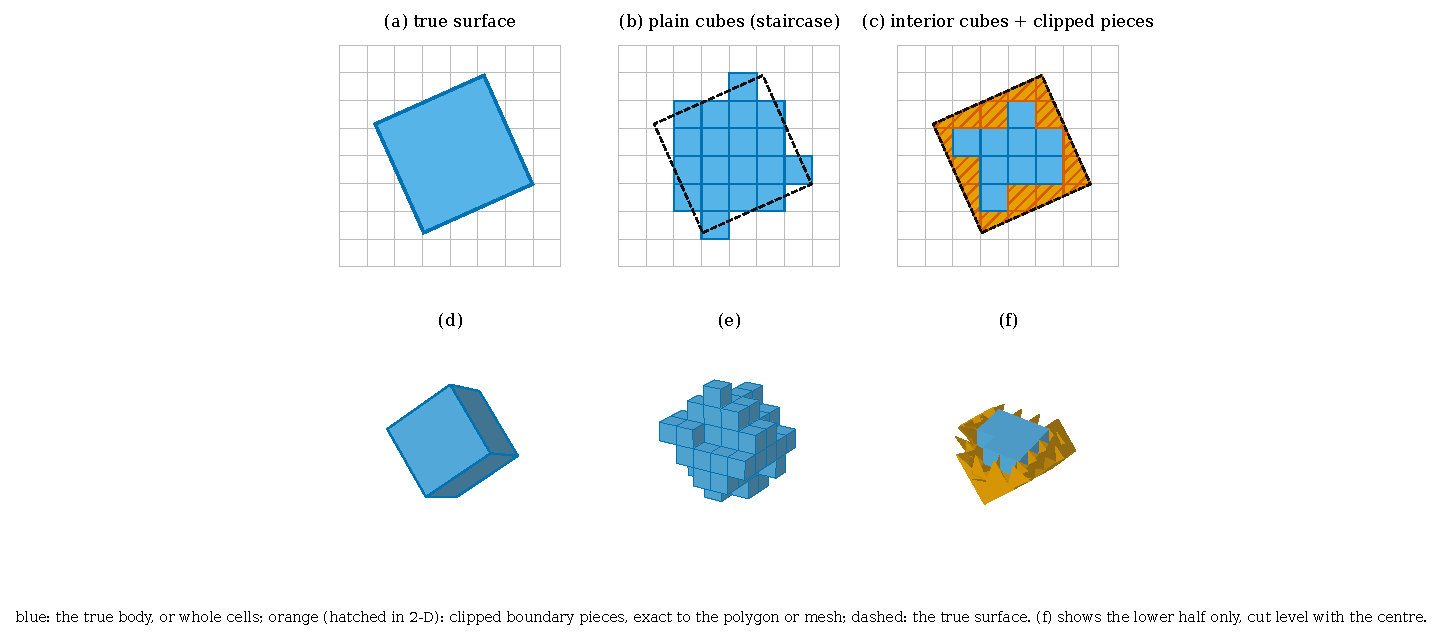
\includegraphics[width=\linewidth]{figures/diag-representations.pdf}
\caption{Three ways to represent a body. Top, a triangle in 2-D; bottom, a square-based
pyramid in 3-D, both on the grid's axes. (a, d) the true surface; (b, e) plain cubes, a cell full when its centre is inside
--- look at the staircase overshooting and undershooting the dotted surface, which is the
first-order error; (c, f) interior cubes plus the clipped boundary pieces, which together are the
body exactly (to the mesh). In (f) the pieces' outlines show where the lattice cuts the faces; the
whole cubes are hidden inside. In (e, f) the true pyramid's edges are dotted, in depth with the
cells: in (e) they pass in front of some steps and behind or inside others. The 3-D panels are lit by a key and a fill light with ambient occlusion, and the bodies stand
on a faint contact shadow.}
\label{fig:repr}
\end{figure}

\paragraph{\Cutcell.} We call a boundary cell that the surface cuts a \emph{cut cell}, as in the
cut-cell methods of computational fluid dynamics. Its scalar \emph{fill fraction} $f$ is the share of
the cell inside the body; \emph{\cutcell} are the mass, centroid and second moment of that filled
part, computed exactly from the clipped piece. The intuition is akin to anti-aliasing in graphics: a
pixel's coverage, rather than a 0/1 decision, removes the jagged edge (Figure~\ref{fig:fill}).

\begin{figure}[!ht]\centering
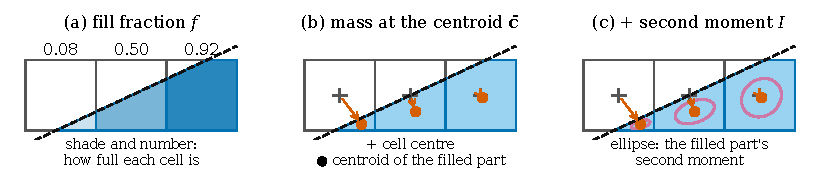
\includegraphics[width=\linewidth]{figures/diag-fill-moments.pdf}
\caption{\Cutcell{} for three cells cut by a surface (dotted; the body below it). (a) The fill
fraction. (b) The mass placed at the centroid of the filled part (dot) rather than the cell centre
(cross): the arrows are the dipole errors a fill fraction at the centre leaves, the first-order
term once the monopole is right; putting the mass at the centroid removes them. (c) The second
moment of the filled part (ellipse, one standard deviation) removes the next term.}
\label{fig:fill}
\end{figure}

\paragraph{Two errors, kept apart.} In this paper \emph{exact} means the analytic shape: a sphere's
field in closed form, a torus's by ring integrals. A triangle mesh is already an approximation of
such a shape, and a clipped piece is exact \emph{to the mesh} only. So a voxelised body carries two
errors that we keep separate throughout: the \emph{facet error}, mesh against analytic shape, which
depends on the triangles and not on the voxels; and the \emph{voxel error}, voxels against the mesh,
which is what the boundary representation controls and what \S\ref{sec:moments} measures. Every
benchmark body here except the sphere is a polyhedron, so for it the two coincide with zero facet
error; the ``sphere' is a 1280-face icosphere, and its errors are measured against the icosphere,
not the sphere. Section~\ref{sec:shapes} measures both errors on curved, scanned and CAD shapes.

\section{The closed form and its derivation}\label{sec:closed}

Take a uniform polyhedron $V$ of density $\rho$ and a field point $\mathbf{p}$ outside it, and write
$\vr = \mathbf{q}-\mathbf{p}$ from the point to the body, $r=|\vr|$. We follow
\citet{werner1997}; \citet{okabe1979} derives the same result by applying the divergence theorem twice
in rotated frames, and \citet{holstein1996} and \citet{tsoulis2012} give line-integral variants.

\paragraph{Volume to faces.} For fixed $\mathbf{p}$ the field $\vr/(2r)$ has divergence (in
$\mathbf{q}$) $1/r$, so by the divergence theorem
\begin{equation}
U \equiv \int_V\frac{dV}{r} = \frac12\oint_{\partial V}\frac{\vn\cdot\vr}{r}\,dS
 = \frac12\sum_f h_f\int_f\frac{dS}{r},\qquad h_f = \vn_f\cdot\vr_f,
\label{eq:faces}
\end{equation}
because $\vn_f\cdot\vr$ is the same for every point of the face's plane: $h_f$ is the signed height
of the plane above $\mathbf{p}$ (Werner \& Scheeres's $\Delta z$). Likewise the attraction
$\mathbf{g}=\int_V\vr\,dV/r^3$ is $-\int_V\nabla_{\mathbf{q}}(1/r)\,dV = -\sum_f\vn_f\int_f dS/r$.

\paragraph{Face to edges.} In the face's plane put the origin at $\mathbf{p}$'s projection, so
$r^2 = x^2+y^2+h^2$. The in-plane field $(x,y)/r$ has divergence $1/r + h^2/r^3$, and Green's
theorem gives
\begin{equation}
\int_f\frac{dS}{r} = \oint_{\partial f}\frac{\hat{\boldsymbol\nu}\cdot(x,y)}{r}\,ds - h\,\omega_f,\qquad
\omega_f \equiv \int_f\frac{h}{r^3}\,dS,
\label{eq:green}
\end{equation}
where $\omega_f$ is the signed solid angle the face subtends at $\mathbf{p}$. Along an edge $e$ with
in-plane outward normal $\hat{\boldsymbol\nu}_e$, the numerator $\hat{\boldsymbol\nu}_e\cdot(x,y)$ is
constant, equal to $\vn_e\cdot\vr_e$ for any point $\vr_e$ of the edge, so the edge contributes
$(\vn_e\cdot\vr_e)\,L_e$ with $L_e = \int_e ds/r$.

\paragraph{The edge integral.} For a segment of length $\ell$ whose ends are at distances $a$ and $b$
from $\mathbf{p}$, and $\mathbf{p}$ off its line,
\begin{equation}
L_e = \int_0^\ell\frac{dt}{\sqrt{(t-t_0)^2+r_0^2}} = \ln\frac{a+b+\ell}{a+b-\ell},
\label{eq:edge}
\end{equation}
from the antiderivative $\ln(t-t_0+r(t))$; the second form follows because
$a^2-t_0^2 = b^2-(\ell-t_0)^2 = r_0^2$.

\paragraph{The solid angle.} For a triangle with vertex offsets $\vr_1,\vr_2,\vr_3$ (anticlockwise
seen from outside), \citet{vanoosterom1983} give
\begin{equation}
\omega_f = 2\,\operatorname{atan2}\bigl(N,\;D\bigr),\quad
N = \vr_1\cdot(\vr_2\times\vr_3),\quad D = r_1r_2r_3 + r_1\,\vr_2\cdot\vr_3 + r_2\,\vr_3\cdot\vr_1 + r_3\,\vr_1\cdot\vr_2.
\label{eq:vos}
\end{equation}
Their derivation rests on the identity
$D^2+N^2 = 2(r_1r_2+\vr_1\cdot\vr_2)(r_2r_3+\vr_2\cdot\vr_3)(r_3r_1+\vr_3\cdot\vr_1)$, whose three
factors are non-negative and vanish only when $\mathbf{p}$ is on a closed edge; so $(D,N)\neq(0,0)$
everywhere else and the $\operatorname{atan2}$ is well defined.

\paragraph{The result, face by face.} Splitting each edge's dyad of \citet{werner1997} between its two
faces, the potential and attraction are
\begin{align}
U &= \frac{G\rho}{2}\sum_f h_f\Bigl(\sum_{e\in f}(\vn_e\cdot\vr_e)L_e - h_f\,\omega_f\Bigr),
&
\mathbf{g} &= -G\rho\sum_f\vn_f\Bigl(\sum_{e\in f}(\vn_e\cdot\vr_e)L_e - h_f\,\omega_f\Bigr),
\label{eq:result}
\end{align}
which is their eqs.~(10) and (15); Figure~\ref{fig:cf} shows the ingredients.

\begin{figure}[!ht]\centering
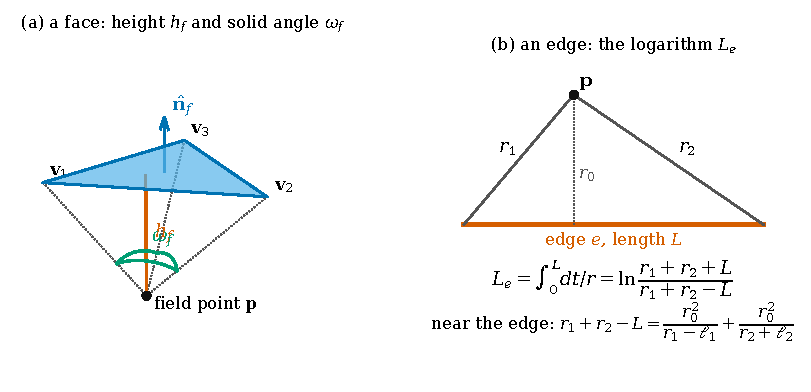
\includegraphics[width=\linewidth]{figures/diag-closed-form.pdf}
\caption{The closed form's ingredients. (a) A face as seen from the field point: its outward normal
$\hat{\mathbf{n}}_f$, the height $h_f$ of its plane above $\mathbf{p}$, and the solid angle $\omega_f$
(green: the face projected onto a small sphere about $\mathbf{p}$). (b) An edge: the distances $r_1,
r_2$ to its ends, its length $L$, and the logarithm $L_e$; the near-edge form avoids subtracting
nearly equal numbers when $r_0$ is small.}
\label{fig:cf}
\end{figure}

\begin{figure}[!ht]\centering
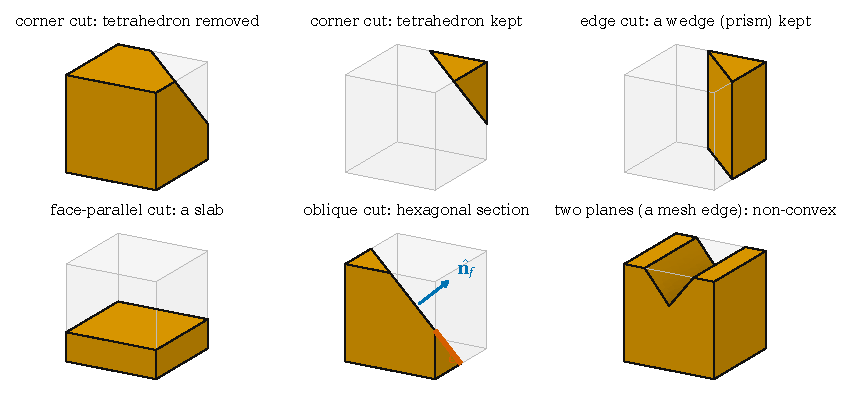
\includegraphics[width=\linewidth]{figures/diag-cuts.pdf}
\caption{One cell, many cuts: the clipped piece (orange) for a corner cut (tetrahedron removed or
kept), an edge cut (a wedge), a face-parallel cut (a slab), an oblique cut through the centre (a
hexagonal section; its face normal $\hat{\mathbf{n}}_f$ and an edge $e$ marked) and two planes meeting
at a mesh edge (a non-convex piece, which the clipper builds as the union of two convex ones; drawn
here as one solid). Each
is a polyhedron, so eq.~(\ref{eq:result}) gives its field exactly to the mesh.}
\label{fig:cuts}
\end{figure} The Laplacian $-G\rho\sum_f\omega_f$ is $0$ outside the body and
$-4\pi G\rho$ inside (their eq.~17): a free check, at every point, that the point is where the scene
says it is. Applied to the field $\vr/r^3$, whose divergence is zero away from $\mathbf{p}$, the same
divergence-theorem step proves the outside half.

\section{Numerical stability}\label{sec:stability}

\paragraph{Far from the body.} With $\gamma = s/R$ the ratio of a body's (or face's) size to its
distance, the field is $O(s\gamma^2)$ while a face term is $O(s\gamma)$, an edge term $O(s)$ and a
vertex term $O(s/\gamma)$; a sum is computed to $\varepsilon$ times its largest term, so the relative
error of a form whose largest terms are of edge size grows as $\varepsilon\gamma^{-2}$ and of vertex
size as $\varepsilon\gamma^{-3}$ or worse \citep[Tables~2--5]{holstein1996}. Equation
(\ref{eq:result}) has edge-sized terms, \emph{provided} two sub-expressions are formed with care.
The edge logarithm must be $L_e=\operatorname{log1p}\bigl(2\ell/(a+b-\ell)\bigr)$, not the ratio of
two numbers that both tend to $2R$. And the solid angle's numerator $N=\vr_1\cdot(\vr_2\times\vr_3)$,
a triple product of vectors of length $R$, carries an absolute error $\varepsilon R^3$ and makes the
face term vertex-sized. But $N = h_f\cdot2A_f$ exactly, the face's height times twice its area, with
$2A_f = |(\mathbf{v}_2-\mathbf{v}_1)\times(\mathbf{v}_3-\mathbf{v}_1)|$ formed from the face's own
edge vectors (\S\ref{sec:lean}, \texttt{numerator\_rule}); written so, it keeps the line-method class.
Figure~\ref{fig:far} shows the three variants on a 1/64~m cube at a non-dyadic position.

\begin{figure}[t]\centering
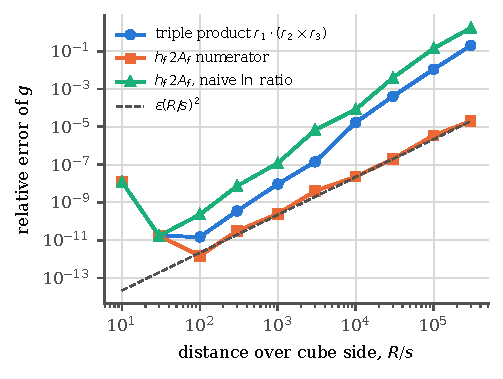
\includegraphics[width=0.48\linewidth]{figures/farfield.pdf}\hfill
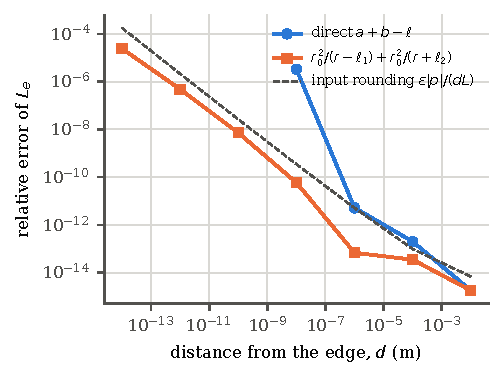
\includegraphics[width=0.48\linewidth]{figures/nearedge.pdf}
\caption{Left: relative error of $\mathbf{g}$ for a 1/64~m cube against its monopole + $l=4$ series,
by distance, for three ways of forming eq.~(\ref{eq:result}); the $h_f\,2A_f$ numerator with
$\operatorname{log1p}$ follows $\varepsilon(R/s)^2$. Right: relative error of $L_e$ at distance $d$
from the middle of a 1/64~m edge; the dashed line is the size of the error that rounding the point's
own position ($\varepsilon|\mathbf{p}|$) can cause, which no formula removes. \provisional}
\label{fig:far}
\end{figure}

\paragraph{Near an edge.} On the segment itself $a+b=\ell$ and $L_e$ is infinite; close to it,
$a+b-\ell$ is a difference of nearly equal numbers. With $\ell_1,\ell_2$ the signed positions of the
ends along the edge from the foot of the perpendicular and $r_0$ the distance to the line,
\begin{equation}
a+b-\ell = \frac{r_0^2}{a-\ell_1}+\frac{r_0^2}{b+\ell_2},
\label{eq:hk}
\end{equation}
which is \citet{holstein1996}'s $r-|\ell| = r_0^2/(r+|\ell|)$ applied at both ends (Okabe's eq.~45
makes the same move). When the point projects onto the segment ($\ell_1\le0\le\ell_2$) both
denominators are sums of non-negative numbers, so nothing cancels. Measured (Figure~\ref{fig:far},
right), the direct form is wrong by $3\times10^{-6}$ at $d=10^{-8}$~m and divides by zero at
$10^{-10}$~m; the form (\ref{eq:hk}) stays at $6\times10^{-11}$ to $10^{-8}$~m, and below that
follows the floor set by rounding the point's position. In $U$ and $\mathbf{g}$ the logarithm is
multiplied by $\vn_e\cdot\vr_e\to0$, so the product is finite and small there.

\paragraph{On the surface.} $U$ and $\mathbf{g}$ are continuous everywhere, on the surface included
\citep{tsoulis2001}; the second derivatives jump across a face and are log-singular on edges. The
correction terms of \citet{tsoulis2001} belong to the line-integral form, where the point's
\emph{projection} falling inside a face, on an edge or on a vertex is singular --- for some face at
almost every point. The solid-angle form (\ref{eq:vos}) is continuous wherever the point is off the
face's plane, and in the plane $\omega_f$ is multiplied by $h_f=0$ in $U$ and $\mathbf{g}$. What
remains degenerate is a point on an edge (above) or at a vertex, where every affected term carries a
vanishing factor. Arm points run in vacuum tubes, so these cases matter for the oracle's own tests.

\paragraph{Against an independent implementation and 40 digits.} ESA's polyhedral-gravity-model
\citep{schuhmacher2024} implements \citet{tsoulis2012}'s line-integral form, so agreement checks the
algebra, not only the code. We ran it (as a tool, writing fixtures; it is GPL-3.0 and is not linked)
on the five benchmark bodies and a non-convex stellated icosahedron, and evaluated
eq.~(\ref{eq:result}) at 40 significant digits on the same f64 vertices to referee
(Figure~\ref{fig:cross}). The pass criterion written beforehand was agreement to $10^{-12}$ at
$R/s\le100$. It holds to $R/s\approx3$ and fails beyond: at 100 body sizes ESA's values are off by
$10^{-10}$--$3\times10^{-8}$ in $\mathbf{g}$, ours by $\le10^{-10}$, so the mismatch is the other
implementation's far-field rounding, in the vertex class as \citet{holstein1996} predict, not an
error in either algebra. Near the body both agree with the 40-digit values to a few $\varepsilon$.

\begin{figure}[t]\centering
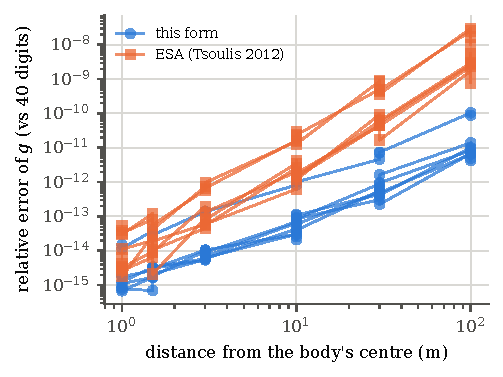
\includegraphics[width=0.55\linewidth]{figures/crosscheck.pdf}
\caption{Relative error of $\mathbf{g}$ against a 40-digit evaluation, worst of three directions,
for six bodies of about 1~m: eq.~(\ref{eq:result}) with the rules of \S\ref{sec:stability}, and ESA's
line-integral implementation. \provisional}
\label{fig:cross}
\end{figure}

\section{\Cutcell: the cheap approximation, measured}\label{sec:moments}

The benchmark lays five convex bodies of about 1~m ($\rho = 2700$~kg\,m$^{-3}$) on lattices of pitch
1/8 to 1/64~m at four random sub-cell placements: a cube with its faces on lattice planes
(\texttt{cube\_aligned}), the same cube turned, an icosahedron, a 1280-face icosphere and a
1~m$\times$1~m$\times$5~cm plate. Each boundary cell is clipped exactly into its piece. Because
interior cubes plus pieces equal the body (checked to $10^{-14}$), the error of any boundary
representation is a sum over boundary cells only, against the exact pieces. The read is the
leading-order gradiometer phase $k_\mathrm{eff}T^2\Delta g_z$ over the 5~m baseline, its lower point
1.5~m and 10~m from the body's centre in three directions. Table~\ref{tab:conv} and
Figure~\ref{fig:conv} give the result.

\begin{table}[t]\centering\scriptsize
\caption{Phase error (rad) at $h=1/64$~m, RMS over four placements of the worst of three directions,
with the least-squares order over $h=1/8$ to $1/64$~m in brackets; read orders to $\pm0.3$. Upper:
1.5~m from the body's centre. Lower: 10~m, with the $h_f\,2A_f$ numerator (with the triple product
the rows below $10^{-9}$ were set by rounding). \provisional}\label{tab:conv}
\begin{tabular}{lrrrrr}
\toprule
representation & cube\_aligned & cube & icosahedron & plate & sphere \\
\midrule
\textit{signal} & \textit{201} & \textit{200} & \textit{214} & \textit{18.3} & \textit{203} \\
0/1 & $3.5\times10^{0}$ (1.0) & $5.6\times10^{-3}$ (2.7) & $1.7\times10^{-2}$ (2.5) & $1.1\times10^{-2}$ (2.3) & $5.1\times10^{-2}$ (1.8) \\
0/1, renormalised & $9.1\times10^{-1}$ (0.9) & $6.5\times10^{-3}$ (2.3) & $5.3\times10^{-3}$ (2.8) & $4.7\times10^{-3}$ (2.3) & $1.3\times10^{-2}$ (2.2) \\
sampled fill $4^3$ (today) & $1.2\times10^{-1}$ (1.2) & $1.2\times10^{-4}$ (2.6) & $2.7\times10^{-4}$ (2.4) & $1.8\times10^{-4}$ (2.5) & $6.8\times10^{-4}$ (2.2) \\
fill fraction & $4.9\times10^{-3}$ (2.0) & $2.5\times10^{-6}$ (3.8) & $1.3\times10^{-5}$ (3.5) & $2.0\times10^{-6}$ (3.8) & $7.6\times10^{-5}$ (2.9) \\
fill + centroid (cube) & $1.0\times10^{-5}$ (3.3) & $1.7\times10^{-5}$ (2.9) & $2.9\times10^{-6}$ (2.9) & $4.2\times10^{-5}$ (2.8) & $6.8\times10^{-7}$ (3.8) \\
fill + centroid (point) & $1.0\times10^{-5}$ (3.3) & $1.7\times10^{-5}$ (2.9) & $2.9\times10^{-6}$ (2.9) & $4.2\times10^{-5}$ (2.8) & $6.8\times10^{-7}$ (3.8) \\
fill + centroid + 2nd moment & $3.9\times10^{-9}$ (4.9) & $4.0\times10^{-7}$ (3.8) & $3.0\times10^{-7}$ (3.9) & $2.6\times10^{-8}$ (3.4) & $2.5\times10^{-7}$ (3.8) \\
\bottomrule
\end{tabular}
\\[6pt]
\begin{tabular}{lrrrrr}
\toprule
representation & cube\_aligned & cube & icosahedron & plate & sphere \\
\midrule
\textit{signal} & \textit{2.89} & \textit{2.89} & \textit{3.09} & \textit{0.282} & \textit{2.93} \\
0/1 & $4.8\times10^{-2}$ (1.0) & $1.2\times10^{-4}$ (2.5) & $2.3\times10^{-4}$ (2.6) & $1.9\times10^{-4}$ (2.3) & $6.8\times10^{-4}$ (1.8) \\
0/1, renormalised & $9.7\times10^{-3}$ (0.9) & $4.2\times10^{-5}$ (2.6) & $4.0\times10^{-5}$ (2.6) & $5.2\times10^{-5}$ (2.3) & $9.1\times10^{-5}$ (2.1) \\
sampled fill $4^3$ (today) & $9.0\times10^{-4}$ (1.3) & $6.6\times10^{-7}$ (2.8) & $1.2\times10^{-6}$ (2.9) & $1.9\times10^{-6}$ (2.7) & $6.1\times10^{-6}$ (2.0) \\
fill fraction & $3.1\times10^{-5}$ (2.2) & $6.3\times10^{-9}$ (4.4) & $8.3\times10^{-8}$ (3.9) & $3.5\times10^{-9}$ (4.2) & $5.8\times10^{-7}$ (3.0) \\
fill + centroid (cube) & $3.2\times10^{-8}$ (3.0) & $3.2\times10^{-9}$ (3.0) & $4.6\times10^{-10}$ (4.2) & $1.3\times10^{-8}$ (2.9) & $2.3\times10^{-10}$ (4.2) \\
fill + centroid (point) & $3.2\times10^{-8}$ (3.0) & $3.2\times10^{-9}$ (3.0) & $4.6\times10^{-10}$ (4.2) & $1.3\times10^{-8}$ (2.9) & $2.3\times10^{-10}$ (4.2) \\
fill + centroid + 2nd moment & $1.2\times10^{-12}$ (4.3) & $8.8\times10^{-12}$ (3.9) & $2.5\times10^{-11}$ (3.9) & $7.6\times10^{-13}$ (4.0) & $2.3\times10^{-11}$ (3.8) \\
\bottomrule
\end{tabular}

\end{table}

\begin{figure}[t]\centering
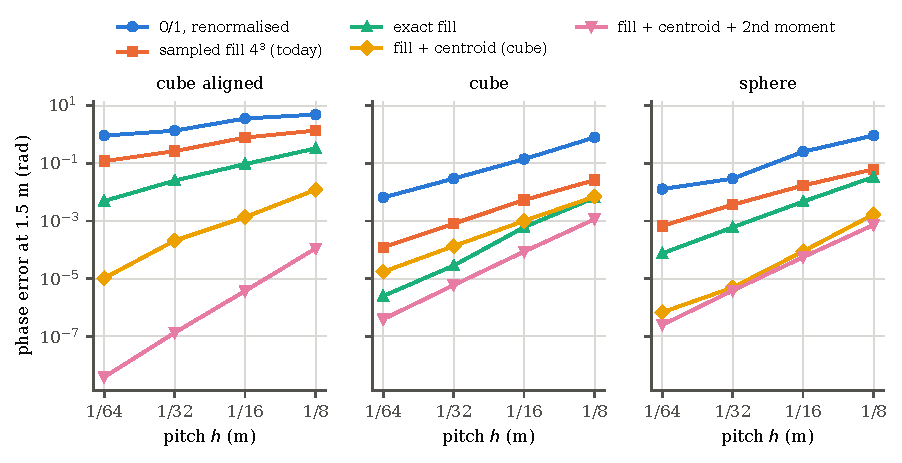
\includegraphics[width=\linewidth]{figures/convergence.pdf}
\caption{Phase error at 1.5~m against pitch, for three bodies. On the aligned cube the sampled fill
(today's Cavendish) is first order; fill + centroid is third order everywhere. \provisional}
\label{fig:conv}
\end{figure}

Three findings. \emph{First}, the worst case is the aligned one: there 0/1 and the sampled fill are
first order and the exact fill second, as Table~\ref{tab:orders} says. \emph{Second}, on turned faces
the exact fill at the cell's centre does better than its bound, order 3.5--4.4. The reason: averaged
over the phase at which a plane of normal $\vn$ cuts a cube, the dipole error is
$-\int_\mathrm{cube}(\mathbf{x}-\mathbf{c})\,\vn\cdot(\mathbf{x}-\mathbf{c})\,dV = -(h^5/12)\,\vn$
for every $\vn$, because a cube's second moment is isotropic; the surface then carries on average a
uniform double layer, and a uniform double layer on a closed surface has no exterior field
($\oint\vn\cdot\nabla(1/r)\,dS = 0$ outside). What remains comes from aligned faces, edges and
curvature. \emph{Third}, the centroid removes the dipole outright but leaves an anisotropic quadrupole
layer that does not cancel, so fill + centroid sits at order 3 everywhere --- worse than the exact
fill on turned faces, but robust; with the second moment as well it is $\ge3.4$ on every body. The
sampled fill of today stays at $10^{-1}$~rad on the aligned cube at 1/64~m; fill + centroid is
$10^{4}$ times better there, and fill + centroid + second moment $10^{7}$ times.

The 10~m rows needed the numerator rule of \S\ref{sec:stability}. With the triple product, the
benchmark's own reference (the sum of the pieces' closed forms, at $R/s\approx600$) is good to only
about $10^{-9}$ relative per piece, and the fill + centroid + second-moment row came out at
$10^{-11}$--$10^{-10}$~rad with orders 2.2--3.7, set by rounding. Rerun with $h_f\,2A_f$, the same row
is $8\times10^{-13}$--$3\times10^{-11}$~rad at orders 3.8--4.3 (Table~\ref{tab:conv}, lower), the
fourth order the analysis predicts; every other row is unchanged to two digits.

\section{Curved, scanned and CAD shapes}\label{sec:shapes}

The benchmark of \S\ref{sec:moments} has five convex bodies with flat faces. This section repeats
the measurement on ten shapes that are none of these: an analytic sphere (radius 1~m) and torus
($R=1$~m, $r=0.4$~m); the Utah teapot and Blender's Suzanne; four scans from the Stanford 3D Scanning
Repository --- the bunny \citep{turk1994}, the dragon and the Happy Buddha \citep{curless1996} and the
Armadillo \citep{krishnamurthy1996}; Keenan Crane's cow Spot \citep{crane2013}; and a mechanical part
from Thingi10K \citep{zhou2016} (file 44950, an extruder drive, public domain), with flat faces, bolt
holes and a fillet. Every mesh body is turned upright and scaled to 1~m largest extent, $\rho =
2700$~kg\,m$^{-3}$. The lower cloud of the tower sits 1.5~m from the surface (or at the stated
distance) along a fixed generic direction, and the read is the leading-order phase of
\S\ref{sec:moments}. The study, its scripts and every number are in
\texttt{docs/research/exact-skin-and-partial-fill.md} \S\S3.1--3.4; \texttt{make.py shapes} draws the
figures and tables here from its committed output (\texttt{scripts/shapes.py}). Every result is
\provisional.

\paragraph{The techniques.} For each boundary cell: (a) a cube, full when its centre is inside;
(b) the sampled fill, $4^3$ points, renormalised to the body's mass (Cavendish today); (c) the exact
fill at the piece's centroid; (d) \cutcell{}, i.e.\ (c) plus the piece's second moment; (e) the
clipped piece itself, exact to the mesh. For the sphere and torus, (c$^\star$) and (d$^\star$) take
each cell's fill, centroid and second moment from the analytic surface directly (the $z$-chords in
closed form, the $(x,y)$ quadrature split at every kink; volumes right to $10^{-13}$--$10^{-11}$), so
no mesh enters at all. Techniques (a)--(e) are measured against the mesh, which is the voxel error of
\S\ref{sec:problem}; (c$^\star$) and (d$^\star$) against the analytic shape --- the sphere's closed
form and, for the torus, a sum of thin rings in complete elliptic integrals over a quadrature of the
cross-section (doubling the quadrature moves the phase by $3\times10^{-14}$~rad).

\paragraph{Meshes, repaired and checked.} The teapot, Suzanne and the bunny are open as downloaded.
They are closed without re-meshing: vertices are welded, back-to-back triangle pairs dropped, each
hole capped by ear clipping its rim, and the parts united in double precision (manifold3d), so every
original triangle is kept. A check with criteria written before measuring --- closed, one piece, every
vertex within $10^{-6}$~m of the original triangles or caps and every original vertex within
$10^{-6}$~m of the result, and no self-crossing (an edge through a triangle by more than $10^{-9}$~m,
the test Cavendish's importer applies) --- passes on every repaired mesh, and its control arm, the
same meshes closed by marching cubes at 1/48~m, fails on every one (by 1.2--4.0~cm, or by a
piece count). The dragon, Armadillo and Buddha have $0.35$--$1.1\times10^{6}$ triangles, too many for
the study's Python clipper, and were decimated (quadric error, then the same repair). The decimation
had its own criterion, also written first: no original vertex further than half the finest pitch,
1/256~m, from the decimated mesh. The Armadillo passes at 60\,000 triangles; \textbf{the dragon and
the Buddha fail} (Table~\ref{tab:decimation}): 691 and 1\,912 original vertices lie beyond 3.9~mm, at
most 2.2 and 1.0~cm away, in thin features under each body that any decimation to this size
collapses (at 150\,000 triangles the dragon's worst vertex is still 2.2~cm away). The tolerance was
not moved. They are used as they are, as what the voxels are measured against; what the decimation
does to the signal is measured below.

\begin{table}[t]\centering\scriptsize
\caption{Decimation against the original scan (same frame, vertex-sampled both ways, exact
point-to-triangle distances). Pass: every original vertex within 1/256~m. The signal change is the
decimated mesh's phase against the full scan's, both summed whole, at 1.5~m. \provisional}
\label{tab:decimation}
\begin{tabular}{lrrrrrrrl}
\toprule
mesh & original & used & \multicolumn{2}{c}{original $\to$ used (m)} & vertices & volume & signal & verdict \\
\cmidrule(lr){4-5}
 & triangles & triangles & max & RMS & beyond 3.9 mm & change & change, 1.5 m (rad) & \\
\midrule
dragon & 871\,414 & 49\,138 & $2.2\times10^{-2}$ & $5.8\times10^{-4}$ & 691 & $-7.1\times10^{-4}$ & $1.1\times10^{-3}$ & \textbf{fail} \\
Armadillo & 345\,944 & 59\,996 & $3.3\times10^{-3}$ & $2.8\times10^{-4}$ & 0 & $-5.7\times10^{-4}$ & $1.3\times10^{-3}$ & pass \\
Buddha & 1\,087\,716 & 47\,974 & $1.0\times10^{-2}$ & $5.0\times10^{-4}$ & 1\,912 & $-3.9\times10^{-4}$ & $6.2\times10^{-4}$ & \textbf{fail} \\
\bottomrule
\end{tabular}

\end{table}

\begin{figure}[t]\centering
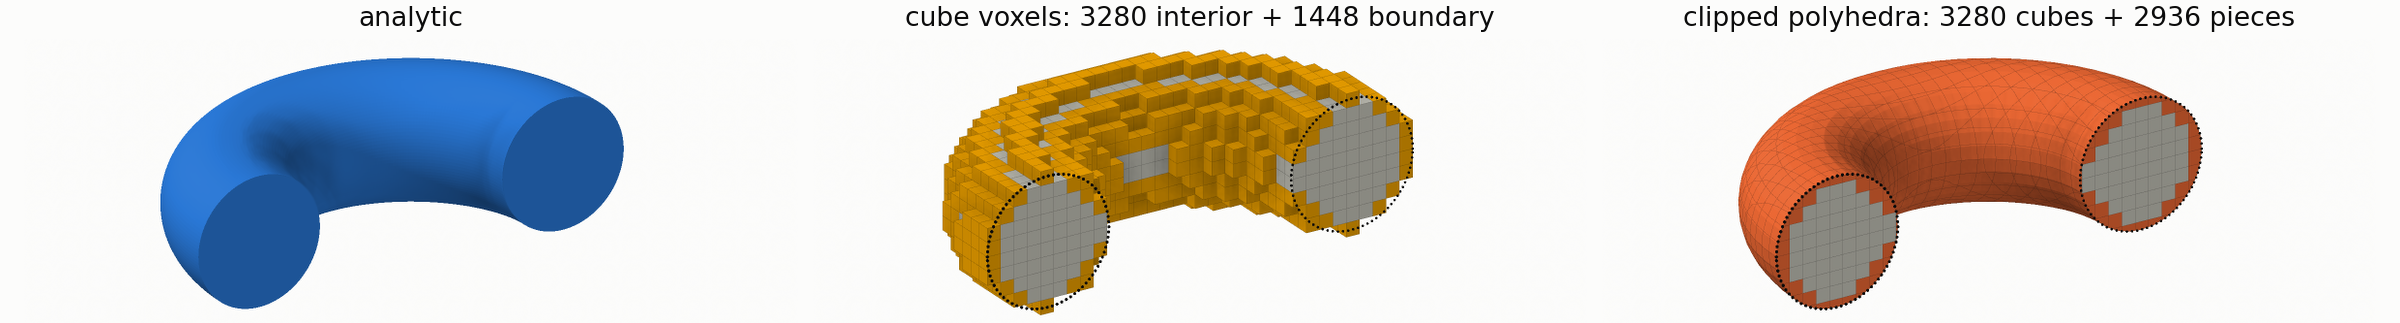
\includegraphics[width=\linewidth]{figures/shapes-torus.png}\\[2pt]
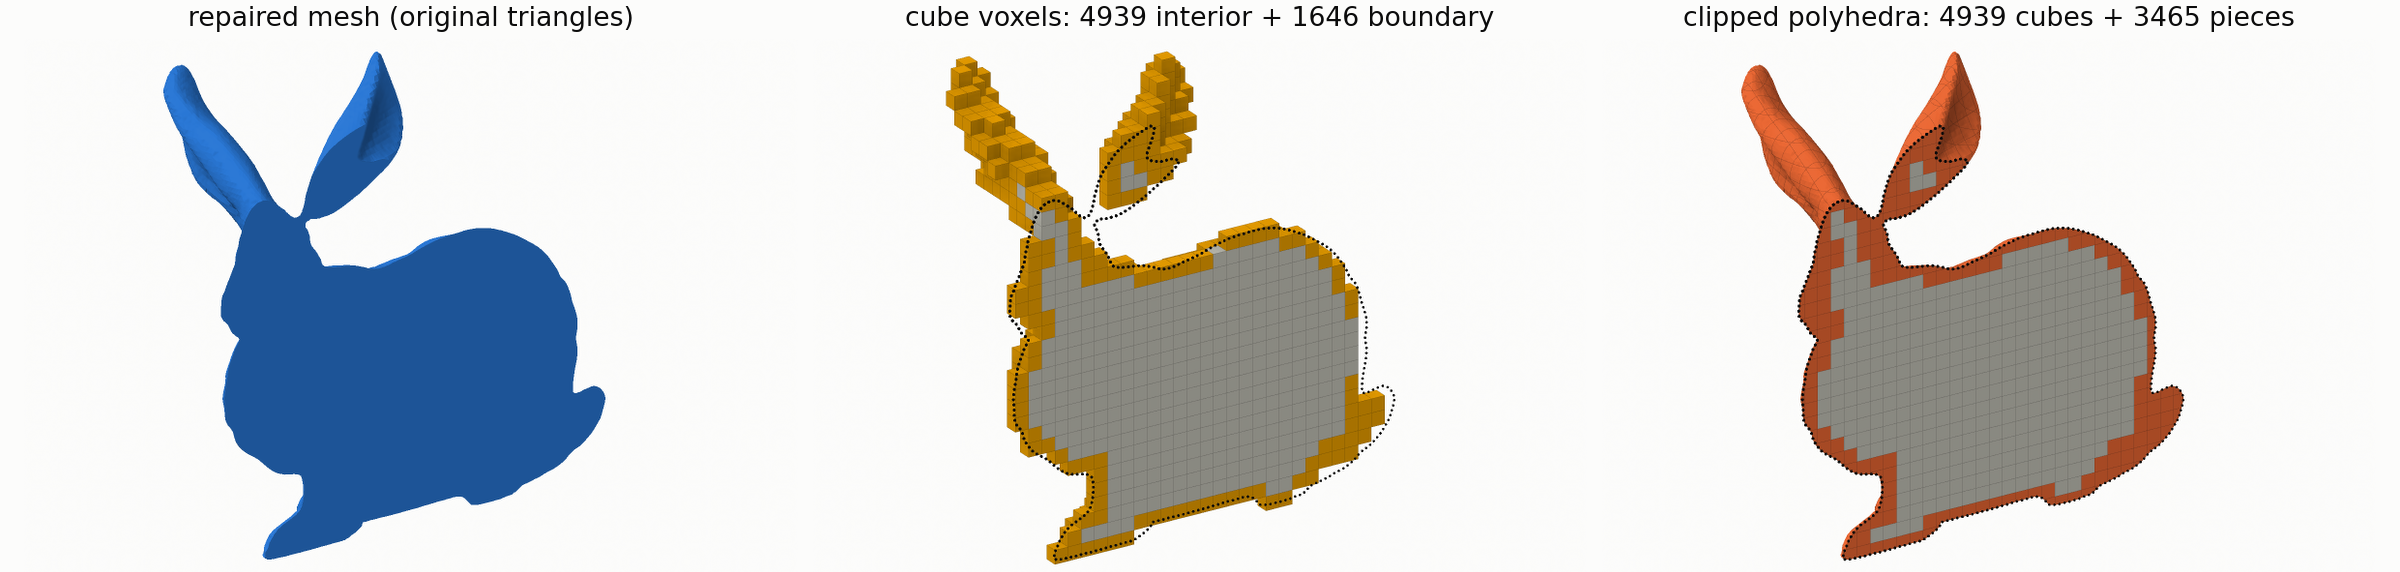
\includegraphics[width=\linewidth]{figures/shapes-bunny.png}
\caption{Two of the ten shapes, each cut away at the lattice wall nearest its centre plane, both at
32 cells across the largest extent. Top: the analytic torus (2.8~m across) at pitch 0.0875~m, whose
cubes and pieces are made from a 4096-triangle mesh; bottom: the Stanford bunny (1~m; 69\,664
triangles, all of the scan's kept, five base holes capped) at 1/32~m. Left, the shape; middle, cubes
full when the centre is inside (grey wholly inside, yellow crossed by the surface); right, the same
interior cubes and every crossed cell clipped to its piece (orange), which together are the body
exactly to the mesh. Dotted: the true surface where the cut meets it, which the cubes' staircase
misses and the pieces follow. The pictures show a lattice four times coarser than the finest one
measured: the sweep runs from 4 to 128 cells across and the errors this section quotes are at 128,
where the cells would be too small to see at print size. Lit as the diagrams are, with screen-space ambient occlusion. Rendered by
the study's \texttt{figures.py}.}
\label{fig:shapes-repr}
\end{figure}

\paragraph{Voxel error against pitch.} Figure~\ref{fig:shapes-sweep} and Table~\ref{tab:shapes-sweep}
take each shape from 4 to 128 cells across. The clipped pieces (e) are at rounding, $\le10^{-11}$~rad,
at every pitch on every shape, and their mass error is $10^{-16}$. \Cutcell{} (d) fall at order
3.6--4.5 on nine of the ten shapes and reach $7\times10^{-11}$ to $10^{-9}$~rad at 128 cells across on
the eight that are meshes in their own right (the teapot to the part); there fill + centroid (c) is
near order 3, at $4\times10^{-8}$ to $2\times10^{-7}$~rad; the sampled fill (b)
has orders from 0.6 to 3.4 and is at $2.5\times10^{-6}$ to $3\times10^{-3}$~rad. The ranking holds with
thin features: on the dragon and the Buddha (d) beats (c) at every pitch, and (c) beats (b) at every
pitch. What thin features change is smoothness. A fold a cell or two across flips in or out of (a)
and (b) as the lattice moves, so they jump by up to ten times from one pitch to the next, while (c)
and (d) carry the exact mass and do not; the Buddha's (d) has a dip at 16 cells across, which brings
its fitted order to 2.9. The CAD part is the case the analysis of \S\ref{sec:moments} predicts to be
worst for sampling and best for moments: its large flat faces lie at fixed heights in the lattice, the
sampled fill's bias does not average out (order 0.6, still $2.7\times10^{-3}$~rad at 128 across), and
(d) is the best of all ten shapes, $7.3\times10^{-11}$~rad at order 4.5.

\begin{figure}[t]\centering
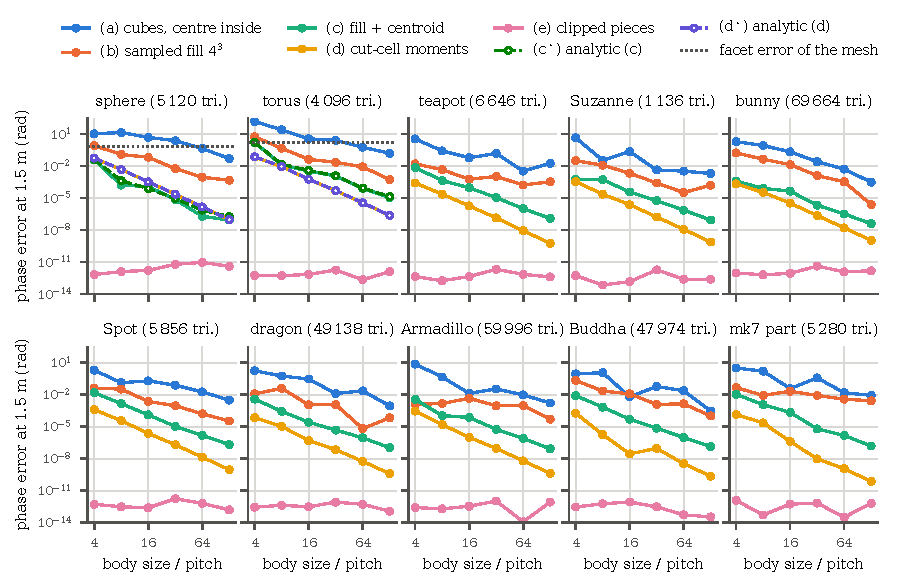
\includegraphics[width=\linewidth]{figures/shapes-sweep.pdf}
\caption{Phase error 1.5~m from the surface against cells across the body, for every technique and
shape. (a)--(e) against the mesh (voxel error); (c$^\star$), (d$^\star$) against the analytic shape;
dotted, the facet error of the mesh used for (a)--(e) on the sphere (5120 triangles) and torus (4096).
Values below $10^{-14}$ are drawn at the axis. \provisional}
\label{fig:shapes-sweep}
\end{figure}

\begin{table}[t]\centering\scriptsize
\caption{Phase error (rad) at 1.5~m with 128 cells across, and in brackets the fitted order in the
pitch over 8 to 128 across; (e) is the largest over all pitches. One tower direction, one lattice
placement per pitch. Upper block: shapes of the study's first part; lower: the scans and the CAD part
(dragon, Armadillo, Buddha decimated). \provisional}
\label{tab:shapes-sweep}
\setlength{\tabcolsep}{3pt}
\resizebox{\linewidth}{!}{\begin{tabular}{lrrrrrrr}
\toprule
shape (triangles) & (a) & (b) & (c) & (d) & (e) & (c$^\star$) & (d$^\star$) \\
\midrule
sphere (5\,120) & $5.2\times10^{-2}$ (2.0) & $4.8\times10^{-4}$ (2.2) & $8.9\times10^{-8}$ (3.1) & $9.6\times10^{-8}$ (3.9) & $\leq$$9\times10^{-12}$ & $1.8\times10^{-7}$ (2.9) & $9.6\times10^{-8}$ (3.9) \\
torus (4\,096) & $1.6\times10^{-1}$ (1.7) & $5.4\times10^{-4}$ (2.2) & $1.1\times10^{-5}$ (2.6) & $2.4\times10^{-7}$ (3.8) & $\leq$$2\times10^{-12}$ & $1.4\times10^{-5}$ (2.6) & $2.4\times10^{-7}$ (3.8) \\
teapot (6\,646) & $1.8\times10^{-2}$ (1.2) & $3.4\times10^{-4}$ (0.9) & $1.2\times10^{-7}$ (3.0) & $5.9\times10^{-10}$ (3.8) & $\leq$$2\times10^{-12}$ &  &  \\
Suzanne (1\,136) & $2.0\times10^{-3}$ (1.4) & $1.6\times10^{-4}$ (1.8) & $9.0\times10^{-8}$ (3.1) & $7.8\times10^{-10}$ (3.7) & $\leq$$2\times10^{-12}$ &  &  \\
\midrule
bunny (69\,664) & $3.1\times10^{-4}$ (2.8) & $2.5\times10^{-6}$ (3.4) & $4.0\times10^{-8}$ (2.9) & $1.1\times10^{-9}$ (3.8) & $\leq$$4\times10^{-12}$ &  &  \\
Spot (5\,856) & $3.1\times10^{-3}$ (1.4) & $3.4\times10^{-5}$ (2.4) & $2.1\times10^{-7}$ (3.2) & $9.1\times10^{-10}$ (3.8) & $\leq$$2\times10^{-12}$ &  &  \\
dragon (49\,138) & $8.7\times10^{-4}$ (2.2) & $6.8\times10^{-5}$ (2.6) & $1.1\times10^{-7}$ (2.7) & $3.9\times10^{-10}$ (3.6) & $\leq$$8\times10^{-13}$ &  &  \\
Armadillo (59\,996) & $1.7\times10^{-3}$ (1.7) & $5.0\times10^{-5}$ (1.2) & $8.4\times10^{-8}$ (2.7) & $4.2\times10^{-10}$ (3.8) & $\leq$$1\times10^{-12}$ &  &  \\
Buddha (47\,974) & $2.9\times10^{-4}$ (2.2) & $1.0\times10^{-4}$ (1.9) & $1.3\times10^{-7}$ (3.0) & $2.3\times10^{-10}$ (2.9) & $\leq$$9\times10^{-13}$ &  &  \\
mk7 part (5\,280) & $8.6\times10^{-3}$ (1.6) & $2.7\times10^{-3}$ (0.6) & $1.5\times10^{-7}$ (3.3) & $7.3\times10^{-11}$ (4.5) & $\leq$$1\times10^{-12}$ &  &  \\
\bottomrule
\end{tabular}
}
\end{table}

\paragraph{The facet error dominates for analytic shapes.} The 5120-triangle icosphere is off from
the sphere by 0.64~rad at 1.5~m and the 4096-triangle torus by 1.8~rad --- more than the plain cubes'
voxel error at 128 cells across. The facet error falls as (triangles)$^{-0.99}$, second order in the edge length: at
81\,920 and 262\,144 triangles the two meshes are still off by 0.04 and 0.03~rad, about $10^{5}$ times
the voxel error of (d) at 128 cells across. For an analytic body, then, the mesh and not the voxels
limits the accuracy, and no boundary representation built from the mesh can do better than the
mesh. Building the cut cells from the analytic surface instead removes the mesh from the chain:
(d$^\star$) is within two digits of (d) at every pitch, so the voxel error does not depend on where
the pieces come from, and the facet error is gone --- the total error of (d$^\star$) against the true
sphere and torus is $10^{-7}$ and $2\times10^{-7}$~rad at 128 across.

\paragraph{An open question: second moments on the sphere.} On the sphere, and only there, adding the
second moment does not help: (d) is worse than (c) at every pitch, by up to 30 times, and the two
meet at 128 cells across. A one-direction result could be a coincidence, so a criterion was written
first: if (d$^\star$) beat (c$^\star$) in RMS over 26 random tower directions, the one-direction
result was a coincidence. It did not. At $h =
0.25$, 0.125 and 0.0625~m the RMS error of (c$^\star$) is $1.7\times10^{-3}$, $5.0\times10^{-5}$ and
$9.0\times10^{-6}$~rad and of (d$^\star$) $4.3\times10^{-3}$, $3.1\times10^{-4}$ and $2.1\times10^{-5}$~rad;
(d$^\star$) wins in 1--2 of the 26 directions. The pieces' summed quadrupole term (RMS $4.0\times10^{-3}$,
$3.5\times10^{-4}$, $1.2\times10^{-5}$~rad) is largely cancelled on the sphere by their higher moments,
which (c) also leaves out, so leaving out both does better than keeping one. On the other nine
shapes (d) beats (c) at every pitch, by 1.4 to 2000 times, and by 23 to 2100 times at 128 across. Why the sphere differs is not explained; adding the pieces'
third moments would test whether the cancellation is between the second and third orders.

\paragraph{Error against cost.} Figure~\ref{fig:shapes-pareto} and Table~\ref{tab:shapes-cost} put a
cost on each point of the sweeps: a direct sum per evaluation point at Cavendish's measured kernel
costs (8.5~ns per cube or point, 17~ns per point and quadrupole, 55~ns per triangle). This is a
\emph{model}, with no tree walk. Within it, (d) is the cheapest voxel route to $10^{-4}$ and $10^{-6}$~rad on
every shape but the sphere (where (c) is, by the anomaly above): on the eight meshes 1.1--13 times
cheaper than (c) at $10^{-4}$~rad and 4--70 times at $10^{-6}$~rad, and on them only (d) reaches
$10^{-8}$~rad within 128 cells across. The inconvenient row is the last:
summing the whole mesh directly is exact to the mesh and, for one body of 1\,000--7\,000 triangles,
cheap. It is cheaper than the clipped pieces on every shape, and at $10^{-8}$~rad cheaper than every
voxel technique except (d) on the teapot (286 against 366~$\mu$s) and the CAD part (48 against
290~$\mu$s). The direct sum loses as the mesh grows: at 50\,000--70\,000 triangles it costs 2.6--3.8~ms
per point, against 0.4--1.4~$\mu$s for (d) at $10^{-4}$~rad. What the model settles is the order within
the voxel techniques, (d) $<$ (c) $\ll$ (b) $<$ (a) per unit of accuracy; the balance against the
direct sum moves towards the voxels with many bodies, large meshes and far points, which a walk
aggregates, and that is not measured here.

\begin{figure}[t]\centering
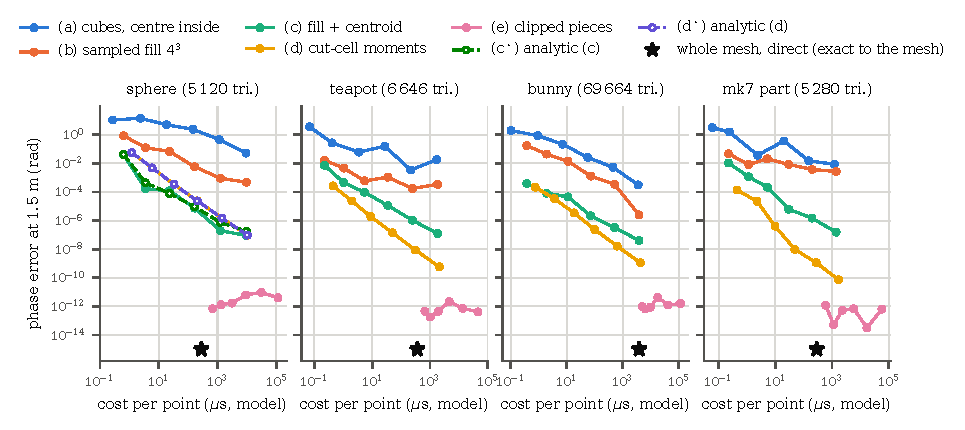
\includegraphics[width=\linewidth]{figures/shapes-pareto.pdf}
\caption{Phase error at 1.5~m against modelled cost per evaluation point, for four of the ten shapes;
points along each line are 4 to 128 cells across. The star is the whole mesh summed directly, exact
to the mesh (drawn at $10^{-15}$). \provisional}
\label{fig:shapes-pareto}
\end{figure}

\begin{table}[t]\centering\scriptsize
\caption{Cheapest modelled cost per evaluation point ($\mu$s) to bring the 1.5~m error below
$10^{-4}$ / $10^{-6}$ / $10^{-8}$~rad within 128 cells across (--- not reached); (e) at 4 across, the
coarsest, which already meets all three. \provisional}
\label{tab:shapes-cost}
\begin{tabular}{lrrrrr}
\toprule
shape & (b) sampled fill & (c) fill + centroid & (d) cut-cell moments & (e) clipped pieces & whole mesh, direct \\
\midrule
sphere & --- / --- / --- & 27 / 510 / --- & 77 / 1\,886 / --- & 690 & 282 \\
torus & --- / --- / --- & 324 / --- / --- & 49 / 1\,164 / --- & 515 & 225 \\
teapot & --- / --- / --- & 5.1 / 259 / --- & 0.81 / 14 / 286 & 674 & 366 \\
Suzanne & 100 / --- / --- & 3.6 / 211 / --- & 1.3 / 19 / 407 & 218 & 62 \\
\midrule
bunny & 844 / --- / --- & 1.6 / 160 / --- & 1.4 / 40 / 893 & 5\,014 & 3\,832 \\
Spot & 673 / --- / --- & 9.9 / 555 / --- & 1.4 / 25 / 582 & 594 & 322 \\
dragon & 65 / --- / --- & 2.1 / 151 / --- & 0.51 / 7 / 175 & 3\,741 & 2\,703 \\
Armadillo & 883 / --- / --- & 1.8 / 157 / --- & 1.2 / 11 / 208 & 4\,328 & 3\,300 \\
Buddha & --- / --- / --- & 2.5 / 133 / --- & 0.36 / 1.9 / 116 & 3\,281 & 2\,639 \\
mk7 part & --- / --- / --- & 7.6 / 280 / --- & 0.59 / 7 / 48 & 597 & 290 \\
\bottomrule
\end{tabular}

\end{table}

\paragraph{Near, middle and far.} Figure~\ref{fig:shapes-regimes} and Table~\ref{tab:shapes-regimes}
move the tower out from the surface to a thousand body sizes, at a fixed pitch, and add two
representations with no voxels at all: (f) the body's own multipole series to $l = 3$ and (g) a point
mass. For each, the table gives the distance beyond which the error stays below $10^{-6}$ and
$10^{-10}$~rad. The clipped pieces are below both from half a cell out on every shape. On the 1~m
bodies at 1/32~m, \cutcell{} are below $10^{-6}$~rad from 0.8--1.2~m and $10^{-10}$~rad from 3--7.3~m;
fill + centroid needs 3--4.7~m and 18--44~m, the body multipole 7--11~m and 28--44~m, a point mass
28--44~m and 167--261~m; the plain cubes reach $10^{-6}$~rad only beyond 100~m and never $10^{-10}$~rad in
range. That is the layering of \S\ref{sec:layers} measured: pieces within about a metre, \cutcell{}
to a few metres, and the body's (or a node's) series beyond. On the sphere (f) and (g) measure the
icosphere's departure from a sphere, and its (d) row is worse than its (c) row, the anomaly above.

\begin{figure}[t]\centering
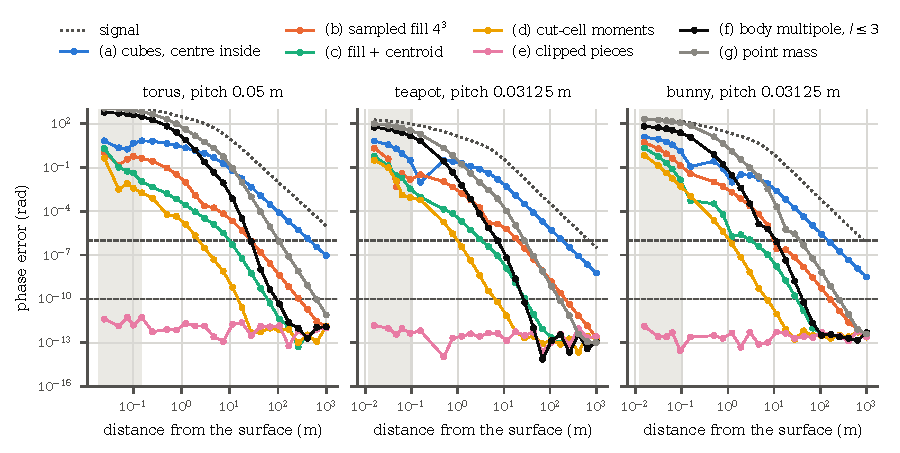
\includegraphics[width=\linewidth]{figures/shapes-regimes.pdf}
\caption{Phase error against distance from the surface, at a fixed pitch, for three shapes; dotted,
the signal; dashed, $10^{-6}$ and $10^{-10}$~rad; shaded, within three cells of the surface. The floor
near $10^{-13}$~rad is rounding. \provisional}
\label{fig:shapes-regimes}
\end{figure}

\begin{table}[t]\centering\scriptsize
\caption{Distance from the surface (m) beyond which each technique's phase error stays below
$10^{-6}$ / $10^{-10}$~rad (--- never, within 1000 body sizes); (e) is below both from half a cell
out everywhere, (a) never reaches $10^{-10}$~rad. Bodies 1~m across except the sphere (2~m) and torus
(2.8~m). \provisional}
\label{tab:shapes-regimes}
\setlength{\tabcolsep}{3.5pt}
\begin{tabular}{lrrrrrrrrr}
\toprule
technique & sphere & torus & teapot & bunny & Spot & dragon & Armadillo & Buddha & mk7 part \\
pitch (m) & 0.0625 & 0.05 & 0.03125 & 0.03125 & 0.03125 & 0.03125 & 0.03125 & 0.03125 & 0.03125 \\
\midrule
(b) sampled fill $4^3$ & 28 / 167 & 28 / 409 & 28 / 261 & 11 / 167 & 18 / 261 & 18 / 167 & 18 / 261 & 28 / 261 & 44 / 409 \\
(c) fill + centroid & 3 / 18 & 11 / 68 & 4.7 / 44 & 4.7 / 44 & 4.7 / 44 & 3 / 44 & 3 / 28 & 3 / 28 & 3 / 18 \\
(d) cut-cell moments & 4.7 / 28 & 3 / 18 & 1.2 / 7.3 & 1.2 / 7.3 & 1.2 / 7.3 & 1.2 / 7.3 & 1.2 / 7.3 & 0.78 / 7.3 & 0.78 / 3 \\
(f) body multipole, $l\leq3$ & 4.7 / 18 & 28 / 107 & 7.3 / 28 & 11 / 44 & 11 / 44 & 11 / 28 & 7.3 / 44 & 11 / 28 & 11 / 44 \\
(g) point mass & 4.7 / 18 & 107 / 639 & 28 / 167 & 44 / 261 & 44 / 261 & 44 / 167 & 44 / 261 & 44 / 167 & 44 / 261 \\
\bottomrule
\end{tabular}

\end{table}

\paragraph{Orientation and motion.} A gradiometer sees bodies move, so the error must not add a
signal of its own. Turned about its axis on a static lattice ($h = 0.1$~m), the torus's (c) and (d)
errors do not change to two digits ($1.2\times10^{-3}$ and $8.6\times10^{-5}$~rad) while the sampled
fill wanders between $5\times10^{-4}$ and $3\times10^{-2}$~rad; a box turned about a generic axis shows
the aligned-face effect of \S\ref{sec:moments} (fill + centroid $1.9\times10^{-5}$~rad aligned,
$10^{-3}$ at $10^\circ$); the teapot's (d) stays at $1.0$--$1.3\times10^{-5}$~rad at every angle.
Moving, the frame of the voxels matters (Figure~\ref{fig:shapes-motion}): the torus passes a tower at
1.5~m closest approach, sampled at $h/16$. Voxelised once in the body's frame and moved rigidly, the
error is smooth and its spectrum has no lines. Re-voxelised on a lattice fixed in the world, it gains
lines at $k/h$ = 10, 20, 30, \dots\ per metre, i.e.\ 10~Hz per m\,s$^{-1}$ of speed, with amplitude at
$1/h$ of 0.22~rad for (a), $2.3\times10^{-4}$ for (b), $3.6\times10^{-7}$ for (c) and $1.0\times10^{-8}$~rad
for (d); the largest error of (d) is $2.8\times10^{-7}$~rad in either frame. Spinning about its axis, the
body-frame error carries harmonics 4 and 8 of the spin and a once-per-turn term ($2\times10^{-2}$~rad
for (a), because the voxelised mass's centre is off the axis; (d) $7\times10^{-8}$~rad peak to peak);
on a world-fixed lattice it repeats with the mesh's 64-fold symmetry, at harmonic 64 of the spin,
$6\times10^{-6}$~rad for (c) and $3\times10^{-7}$~rad for (d). Cavendish stores bodies in their own
frame, which avoids the lines.

\begin{figure}[t]\centering
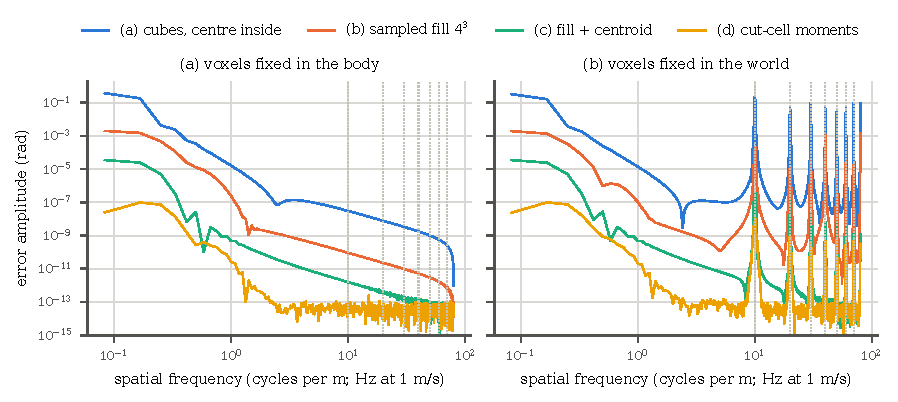
\includegraphics[width=\linewidth]{figures/shapes-motion.pdf}
\caption{Spectrum of the phase error as the torus passes a tower at 1.5~m ($h = 0.1$~m): (a) voxels
fixed in the body, (b) voxels fixed in the world and re-made as it moves; dotted, multiples of
$1/h$. Spatial frequency is a temporal one in Hz at 1~m\,s$^{-1}$. \provisional}
\label{fig:shapes-motion}
\end{figure}

\paragraph{What a cell is drawn as matters little; where it sits matters.} Given each cell's exact
piece mass, the primitive that carries it --- a point at the cell's centre, a uniform sphere or cube,
the cube's series, a Gaussian, a trilinear density --- gives the same error to the digit beyond about
two cells (teapot, $h = 1/16$~m: $9\times10^{-3}$~rad at 10 cells, $10^{-5}$ at 100). A point at the
piece's centroid is 7--100 times better at every distance, and the clipped piece is at rounding.

\paragraph{Full resolution, in Cavendish.} The scans were also given whole to Cavendish's own importer
and voxeliser (release build, one thread; caps unchanged). The bunny as downloaded is refused as open
(223 edges not in exactly two triangles once each way: its base holes); closed, it imports in 0.18~s.
\textbf{The full dragon and Buddha are refused}: as STL files (43.6 and 54.4~MB) at the importer's
32~MiB byte cap, and given as arrays at its 500\,000-triangle cap (871\,306 and 1\,087\,422 triangles);
Lucy (28 million triangles) would be refused at both. The caps were not changed for the test; whether
they should be is a decision for the engine. What was accepted imports at 2.6--4.6~$\mu$s per triangle
and voxelises to 1/128~m in 0.5--27~s in under 100~MiB; the tree depends on the shape and not the
triangle count (43\,039 leaves for the full Armadillo, 42\,665 for its decimation). The direct
whole-mesh sum costs 53--67~ns per triangle per point from 5\,000 to a million triangles, so a
whole-mesh read is 0.07~s per point for the Buddha and, extrapolated, 1.7~s for Lucy --- at every
sampled time of every cloud of every tower. Voxelised once, the same body read through the tree and
\cutcell{} costs what its leaves cost, which does not grow with the triangles. (The study's Python
clipper does run on the full meshes: 0.7--4~million piece triangles, volumes adding to the mesh's to
$10^{-15}$.)

\paragraph{Each mesh as one polyhedron.} With no voxels at all, each body is its mesh and its field is
eq.~(\ref{eq:result}) summed over every triangle; its mass moments follow from the same triangles by
the divergence theorem. Both are exact to the mesh; the phase is still the leading-order one at one
instant. Figure~\ref{fig:shapes-exact} and Table~\ref{tab:shapes-exact} give what a tower reads.
Beyond about 2~m every body reads like its mass: a point mass is off by 3--40\% at 1.5~m, 0.05--0.6\%
at 5~m and $3\times10^{-5}$--$8\times10^{-4}$ at 20~m; the second moments bring 20~m to
$2$--$8\times10^{-6}$ and the third to $0.5$--$2\times10^{-7}$. Inside about 2~m the series does not
converge usefully and the shape takes over: the bunny, Spot and the dragon show a sign change near
1~m, where the body's mass, uneven above and below the level of the lower cloud, pulls it vertically
harder than it pulls the upper one. The decimated dragon, Armadillo and Buddha differ from the full
scans by a nearly constant 4--7$\times10^{-4}$ of the signal at every distance --- their mass change ---
which at 1.5~m is $0.6$--$1.3\times10^{-3}$~rad (Table~\ref{tab:decimation}), about a million times the
voxel error of (d) against the decimated mesh. As with the facet error of the analytic shapes, the
mesh, not the voxels, limits the accuracy: a body must be meshed to the accuracy wanted before its
voxels can deliver it. Walking past at 1.4~m\,s$^{-1}$ and 2~m from the axis, the same body in three
poses gives peaks differing by 4--18\%, far above any instrument floor, most for the bodies with a
long axis turned towards the tower: a gradiometer that sees a walker-sized body pass at 2~m sees its
shape, not only its mass.

\begin{figure}[t]\centering
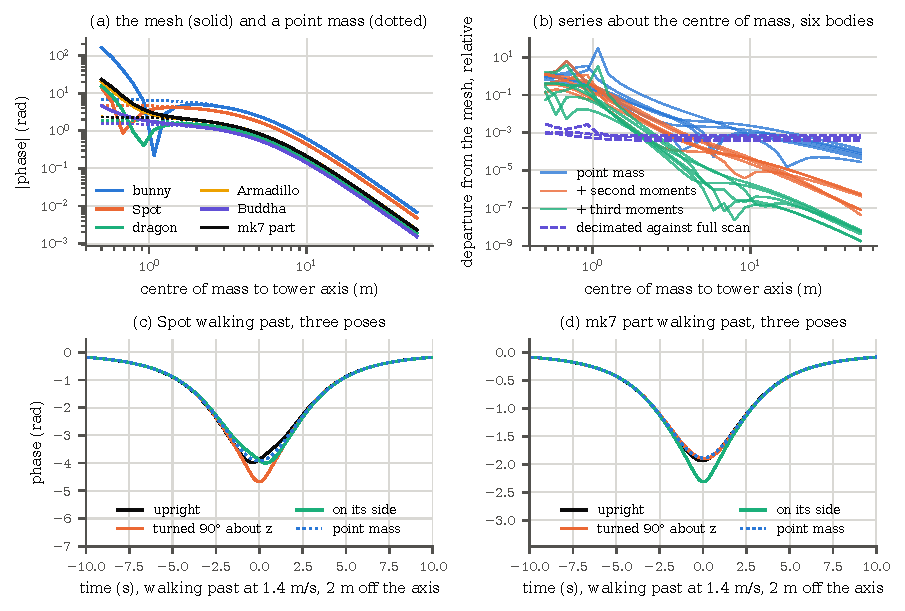
\includegraphics[width=\linewidth]{figures/shapes-exact.pdf}
\caption{Each mesh as one polyhedron, its field summed over every triangle (exact to the mesh). (a)
Phase against the distance from the centre of mass to the tower's axis, level with the lower cloud.
(b) How far the series about the centre of mass (point mass; with second; with third moments) depart
from it, for all six bodies; dashed, the decimated meshes against the full scans. (c, d) Walking past
at 1.4~m\,s$^{-1}$, 2~m from the axis, in three poses, and the point mass. \provisional}
\label{fig:shapes-exact}
\end{figure}

\begin{table}[t]\centering\scriptsize
\caption{Each mesh as one polyhedron: mass (from the mesh), peak phase walking past in three poses
and as a point mass, the largest difference between poses at any one time, and the point mass's
relative departure from the mesh's field at 1.5, 5 and 20~m. \provisional}
\label{tab:shapes-exact}
\setlength{\tabcolsep}{4pt}
\begin{tabular}{lrrrrrrrr}
\toprule
mesh & triangles & mass (kg) & \multicolumn{4}{c}{peak phase walking past (rad)} & poses differ & point mass off by \\
\cmidrule(lr){4-7}
 & & & upright & turned & on side & point mass & by up to & 1.5 / 5 / 20 m \\
\midrule
bunny & 69\,664 & 540.0 & 5.00 & 5.52 & 5.53 & 5.54 & 0.55 (10\%) & $4\times10^{-1}$ / $6\times10^{-3}$ / $3\times10^{-5}$ \\
Spot & 5\,856 & 382.5 & 3.98 & 4.68 & 4.00 & 3.92 & 0.84 (18\%) & $4\times10^{-2}$ / $2\times10^{-3}$ / $5\times10^{-4}$ \\
dragon & 49\,138 & 150.0 & 1.49 & 1.50 & 1.54 & 1.54 & 0.06 (4\%) & $1\times10^{-1}$ / $5\times10^{-4}$ / $3\times10^{-4}$ \\
Armadillo & 59\,996 & 185.3 & 1.92 & 2.03 & 1.93 & 1.90 & 0.13 (6\%) & $3\times10^{-2}$ / $5\times10^{-4}$ / $3\times10^{-4}$ \\
Buddha & 47\,974 & 123.1 & 1.29 & 1.24 & 1.26 & 1.26 & 0.05 (4\%) & $6\times10^{-2}$ / $1\times10^{-3}$ / $5\times10^{-4}$ \\
mk7 part & 5\,280 & 184.3 & 1.94 & 1.90 & 2.31 & 1.89 & 0.41 (18\%) & $7\times10^{-2}$ / $4\times10^{-3}$ / $8\times10^{-4}$ \\
\bottomrule
\end{tabular}

\end{table}

\FloatBarrier
\section{The octree}\label{sec:octree}

Cavendish stores each body as a sparse octree in the body's own frame. Eight equal children merge
losslessly into their parent, so a body's interior collapses into the largest cubes that lie wholly
inside it (Figure~\ref{fig:tree}). Cut cells never merge: each carries its own moments, and no two
are equal, so they stay at the finest level. The tree's leaves therefore grow as the surface,
$\propto N^2$ for $N$ cells across, while a uniform grid grows as $N^3$. Counted for a sphere
(Figure~\ref{fig:storage}, \texttt{data/storage.json}): at $N = 256$ cells across the root the
uniform grid holds $4.3\times10^{6}$ cells in or cut, the octree $3.1\times10^{5}$ leaves (14 times
fewer), of which $1.9\times10^{5}$ are cut cells; the ratio doubles with each doubling of $N$.

\begin{figure}[!ht]\centering
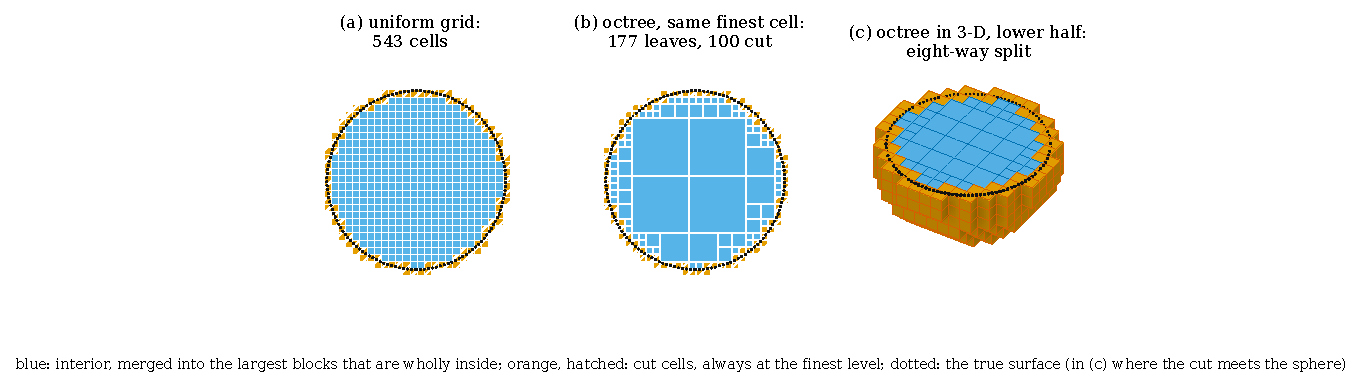
\includegraphics[width=\linewidth]{figures/diag-tree.pdf}
\caption{The same body as a uniform grid and as an octree with the same finest cell. (a, b) A
cross-section through each; (c) the octree in 3-D, lower half, showing the eight-way split. Look at
the interior: one large block where the grid has hundreds of cells; the cut cells (orange) stay at
the finest level. In (c) the sphere's rim at the cut is dotted.}
\label{fig:tree}
\end{figure}

\begin{figure}[!ht]\centering
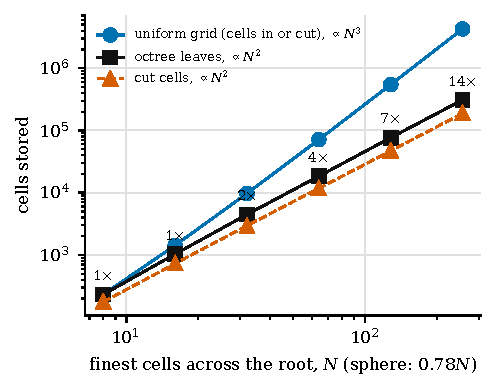
\includegraphics[width=0.55\linewidth]{figures/diag-storage.pdf}
\caption{Cells stored against cells across the root for a sphere: the uniform grid ($\propto N^3$),
the octree's leaves and the cut cells (both $\propto N^2$); numbers are the grid-to-octree ratio.
Counted by \texttt{scripts/octree\_diagrams.py}.}
\label{fig:storage}
\end{figure}

\paragraph{Node moments are the true body's.} A node's moments (mass, centroid, second and higher
moments) are the sums of its children's, moved to its centre by the parallel-axis rule. With
\cutcell{} at the leaves, every node's moments are those of the body as the mesh defines it, not of
the voxel staircase; so the far field read from coarse nodes is the mesh's far field, and the only
error a coarse node adds is the truncation of its multipole series.

\paragraph{The read.} For each tower the read walks the tree in the manner of
\citet{barnes1986}, but a node is accepted when a rigorous bound on its error in the
\emph{phase} is below its share of the tolerance, rather than by a fixed opening angle; error-based
opening is what avoids the long error tails of an angle criterion \citep{salmon1994,dehnen2014}. The
accepted nodes form a cut through the tree (Figure~\ref{fig:readcut}). Measured in Cavendish's S5
research note on a 128$^3$-cell town (\provisional): with a geometric criterion the nearest accepted
node of each level sits 2.6--5.7 node sides from the tower, so each level forms a ring about three
nodes wide; per tower per shot (40 points) the leaf-by-leaf read costs $6.5\times10^{6}$
interactions, a per-point walk $1.9\times10^{4}$, and a shared cut with a local expansion about the
tower $\approx3\times10^{3}$. The rigorous bound is loose: Cavendish's is 27--457 times the true
error, and \citet{salmon1994}'s bound on a uniform cube, with exact absolute moments, is 109--4800
times the true remainder at order $p=1$, 38--350 at $p=2$ and 6--65 at $p=3$ --- intrinsic to an
absolute, per-node bound (a cube's low multipoles vanish), compounded by adding node bounds with the
triangle inequality ($\sum|e_i|/|\sum e_i| = 3$--27 on the town's cut). The gradiometer's 5~m
baseline helps only modestly: the difference bound lets a node be accepted at about 0.7 times the
distance at 100~m and 0.5 times at 1~km, and gains nothing on the town, whose nodes are within ten
baselines.

\paragraph{Scaling.} Storage is $\propto N^2$ leaves plus 8--20 bytes of \cutcell{} per cut cell;
the read's cost per point grows with the number of levels times the nodes per ring, about
$\log_2 N$ times a constant, rather than with $N^3$ (derived, not measured).

\section{The layered scheme and its error budget for AION-10}\label{sec:layers}

The closed form and the moments are complementary. The closed form is exact but costs about 55~ns per
triangle and point on one thread (a clipped cell has 7--14 triangles) and loses accuracy as
$\varepsilon(R/s)^2$ with distance; a piece's moments cost little and lose accuracy as $(h/d)^k$ with
nearness. So Cavendish layers them, as it already layers Nagy's prism (near) and the cube's series
(far):
\begin{enumerate}\itemsep0pt
\item \textbf{Near} (within a few cells of an arm point): the clipped piece, eq.~(\ref{eq:result}), exact to the mesh.
\item \textbf{Middle}: \cutcell{} --- each cut cell's mass, centroid and second moment; interior
 leaves are full cubes ($f=1$, $\bar{\mathbf{c}}=\mathbf{c}$, $I = (h^2/12)\,\mathbf{1}$).
\item \textbf{Far}: the octree walk, whose nodes carry the sums of their leaves' moments --- now the
 true body's moments rather than the staircase's --- opened by a bound on the phase error.
\end{enumerate}
Because the phase (\ref{eq:phase}) is a linear functional of $V$, and the pieces partition the body,
the layers add without any error of their own: the phase of the body is the sum of the phases of its
pieces, and the quadrature error of the whole is the sum of the pieces' quadrature errors
(\S\ref{sec:lean}, \texttt{quadrature\_error\_additive}). Figure~\ref{fig:readcut} shows the
layers as the read's cut through the octree, and Table~\ref{tab:budget} is the budget.

\begin{figure}[!ht]\centering
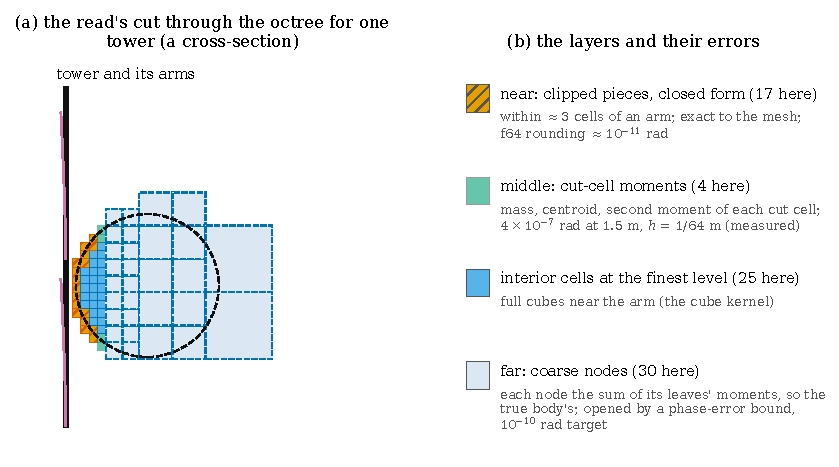
\includegraphics[width=\linewidth]{figures/diag-read-cut.pdf}
\caption{The layered read, as a cross-section through the octree for one tower (schematic: the
acceptance rule here is a node side at most half its distance from the arm, and ``near'' is three
cells; Cavendish opens nodes by a bound on the phase error). Look at how the nodes grow with
distance from the arm: clipped pieces only beside it, \cutcell{} a little further, and beyond that
single nodes standing for many cells, each carrying the sums of its leaves' moments.}
\label{fig:readcut}
\end{figure}

\begin{table}[t]\centering\small
\caption{Error budget for one AION-10 read of a tonne-scale body 1.5~m from the lower arm, pitch
1/64~m, worst body of the benchmark. Measured rows are from Table~\ref{tab:conv} and
Figure~\ref{fig:cross} (relative error of $\mathbf{g}$ at $\le1.5$~m times the largest signal,
$\SignalMax$~rad); design rows are Cavendish's tolerances. \provisional}\label{tab:budget}
\begin{tabular}{lrl}
\toprule
contribution & phase (rad) & source \\
\midrule
boundary cells as sampled fill $4^3$ (Cavendish today) & $1.2\times10^{-1}$ & measured \\
boundary cells as fill + centroid & $4.2\times10^{-5}$ & measured \\
boundary cells as fill + centroid + second moment & $4.0\times10^{-7}$ & measured \\
closed form, whole body or clipped pieces (f64 rounding) & $8.2\times10^{-12}$ & measured \\
octree far field (S5 walk tolerance) & $1.0\times10^{-10}$ & design \\
flight quadrature (audited read, \texttt{PHASE\_TOLERANCE}) & $1.0\times10^{-10}$ & design \\
shot-noise floor, rad\,Hz$^{-1/2}$ (AION-10 baseline, for scale) & $1.0\times10^{-4}$ & reference \\
\bottomrule
\end{tabular}

\end{table}

The representation of the boundary is the only row that the choice of this paper moves: from
$10^{-1}$~rad today to a few $10^{-7}$~rad with second moments, with the clipped pieces taking the
nearest cells to rounding. All of these are voxel errors, against the mesh; the facet error of a mesh
that stands in for a curved shape is separate and is not in this table: it is $0.6$~rad for a
5120-triangle sphere and $10^{-3}$~rad for a decimated scan (\S\ref{sec:shapes}), unless the cut cells
are taken from the analytic surface. The far and quadrature rows are held at $10^{-10}$~rad by the walk's bound
and the audited read; the closed form's own rounding is negligible at the distances where it is used.

\section{The Lean formalisation}\label{sec:lean}

The derivation of \S\ref{sec:closed} is formalised in Lean~4 \citep{moura2021} with Mathlib
\citep{mathlib2020} (\texttt{proofs/polyhedral-gravity/}, Lean v4.36.0, Mathlib v4.36.0). There is no
\texttt{sorry} and no \texttt{axiom}: \texttt{\#print axioms} on every main theorem lists only Lean's
standard three (\texttt{propext}, \texttt{Classical.choice}, \texttt{Quot.sound}), and what is not
proven is an explicit hypothesis of the theorem that uses it. Table~\ref{tab:lean} lists the
statements.

\begin{table}[!ht]\centering\small
\caption{What is machine-checked, and what is assumed.}\label{tab:lean}
\begin{tabular}{p{0.37\linewidth}p{0.57\linewidth}}\toprule
statement (Lean name) & status\\\midrule
edge integral (\ref{eq:edge}), any real inner-product space (\texttt{edge\_integral}) & proven, by FTC
from the antiderivative; point off the edge's line\\
log1p form and near-edge form (\ref{eq:hk}) (\texttt{edge\_integral\_log1p}, \texttt{gap\_near\_edge\_vec}) & proven\\
numerator rule $N = h_f\,2A_f$; height the same from every vertex (\texttt{numerator\_rule}, \texttt{height\_const}) & proven\\
$D^2+N^2 = 2\prod(r_ir_j+\vr_i\cdot\vr_j)$, factors $\ge0$ (\texttt{vos\_modulus}, \texttt{vos\_ne\_zero}) & proven\\
Van Oosterom--Strackee formula (\ref{eq:vos}) itself & \textbf{cited, not proven}; $\omega_f$ is
\emph{defined} as $\int_f h/r^3\,dS$\\
divergences: $\nabla\cdot(\vr/2r)=1/r$, $\nabla\cdot(\vr/r^3)=0$, in-plane $1/r+h^2/r^3$, $\nabla\cdot(\hat{\mathbf{e}}_k/r)$ (\texttt{Divergence.lean}) & proven, with explicit derivatives\\
box: $U$, $\mathbf{g}$ to face integrals, $\sum$ solid angles $=0$ (\texttt{box\_potential}, \texttt{box\_attraction}, \texttt{box\_gauss}) & proven from Mathlib's divergence theorem on boxes: \textbf{no hypotheses}\\
box faces: a rectangle's $\int dS/R$ = edge terms $- h\,\omega$; each rectangle edge in closed form
(\texttt{rect\_face}, \texttt{rect\_edge}) & proven from Mathlib's divergence theorem in the plane:
\textbf{no hypotheses}; the substitution of these into \texttt{box\_potential} is not written out as
one theorem (index bookkeeping only)\\
general polyhedron: eqs.~(\ref{eq:result}) and $\sum_f\omega_f=0$ outside (\texttt{potential\_faces\_edges}, \texttt{attraction\_faces\_edges}, \texttt{solid\_angles\_sum\_zero}) & proven \textbf{given} the divergence theorem for $V$ and Green's theorem on each face, stated as hypotheses; frames orthonormal (Parseval stated as a field); point outside a compact set holding the body and off every edge's line\\
$\sum_f\omega_f = 4\pi$ inside & \textbf{not proven}\\
pieces sum to the body; phase and its quadrature linear; exact pieces give the exact quadrature phase
(\texttt{Superposition.lean}) & proven\\\bottomrule
\end{tabular}
\end{table}

Two remarks. Mathlib's divergence theorem is stated for boxes in $\mathbb{R}^{n+1}$, so a rectangular
box --- Nagy's prism, the cube kernel of every interior voxel --- needs no hypothesis for the
volume-to-faces step; the general polyhedron does, and we state it in the form of a theorem
quantified over all fields differentiable on a neighbourhood of the body, so that it is the classical
statement and not something tailored to these fields. And Mathlib's norm on $\mathrm{Fin}\,n\to\mathbb{R}$
is the supremum norm, so every distance in the formalisation is written out as
$\sqrt{\sum_j(q_j-p_j)^2}$; the edge integral is stated in an arbitrary real inner-product space and
so covers $\mathbb{R}^3$ with its Euclidean norm directly.

\section{Limitations}\label{sec:limits}

\begin{itemize}\itemsep0pt
\item Every number here is from the Python benchmark, not from Cavendish; all are provisional until
S5 regenerates them. The benchmark of \S\ref{sec:moments} has convex bodies; the non-convex shapes of
\S\ref{sec:shapes} were measured with one tower direction and one lattice placement per pitch, so
their fitted orders are rougher than Table~\ref{tab:conv}'s.
\item Curved analytic shapes are not polyhedra. Their \cutcell{} can be taken from the surface
directly (\S\ref{sec:shapes}, sphere and torus); their exact clipped pieces were not built, and near a
tower the stand-in is a mesh, whose facet error dominates.
\item Why second moments make the sphere worse is open (\S\ref{sec:shapes}).
\item The costs of \S\ref{sec:shapes} are a model of a direct sum with measured kernel costs, with no
tree walk; Cavendish's importer, at its present caps, refuses the full dragon and Buddha, and the
decimations used instead fail their own criterion.
\item The read in \S\ref{sec:moments} is the leading-order $k_\mathrm{eff}T^2\Delta g_z$, not
Cavendish's full flight integral (\ref{eq:phase}); the orders do not depend on this, the prefactors
slightly do.
\item The cost of exact clipping in compiled code (estimated $10^{-6}$--$10^{-5}$~s per cell) is not
measured; the f32 behaviour of the closed form on the GPU is derived from the scaling, not measured.
\item In Lean: the divergence and Green theorems for general polyhedra are hypotheses; the
Van Oosterom--Strackee formula is cited; the inside value $4\pi$ and points on an edge's extension
(where $L_e$ is finite but $r_0=0$) are not covered; the derivation is for the attraction integral
$\int\vr/r^3\,dV$, and that it equals $\nabla U$ (differentiation under the integral) is not
formalised.
\end{itemize}

\appendix
\section{Reproducing this paper}\label{app:repro}
\texttt{python make.py all} reruns everything from the stored benchmark and shapes-study output;
\texttt{python make.py shapes-study} reruns the shapes study itself (hours; it downloads the meshes,
checked against pinned SHA-256 hashes); \texttt{python
make.py bench} reruns the benchmark itself (about 40 minutes on one core); \texttt{python make.py esa
<venv-python>} reruns the ESA fixtures in their own environment. The Lean proofs build with
\texttt{lake exe cache get \&\& lake build} in \texttt{proofs/polyhedral-gravity}. The paper's
\texttt{README.md} lists, for each table and figure, the Cavendish command that is to replace the
script once S5 lands, and the scene file in \texttt{scenes/} it reads.

\begin{figure}[!ht]\centering
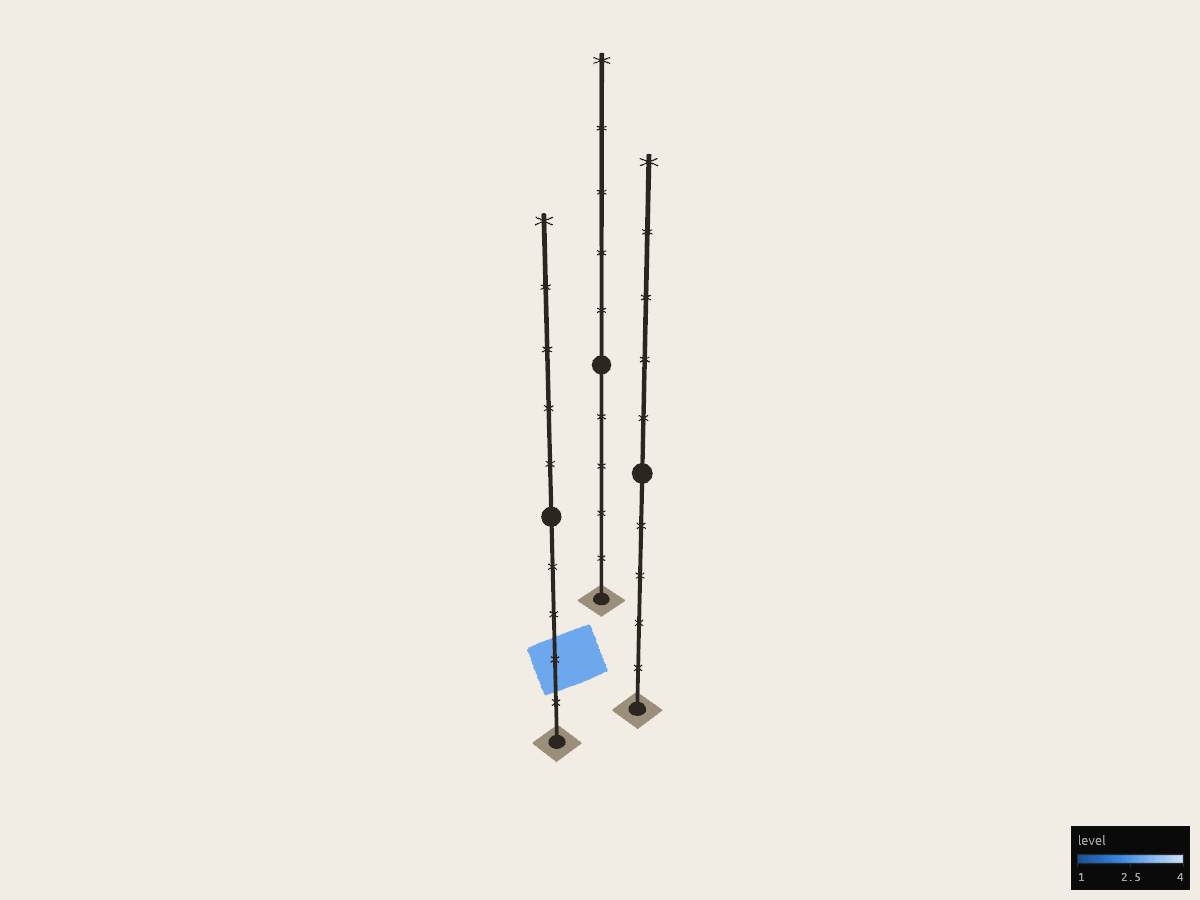
\includegraphics[width=0.45\linewidth]{figures/scene-cube-1.5m.png}
\caption{The benchmark's turned cube as a Cavendish scene (\texttt{scenes/cube-1.5m.ron}: the
body's exact triangles held in the scene, three towers 1.5~m from its centre), drawn by
\texttt{cav render}. Today Cavendish voxelises it with the sampled fill; S5 adds the representations
of Table~\ref{tab:orders} as a field of the body.}
\label{fig:scene}
\end{figure}

\section{The Python cross-check}\label{app:python}
The research benchmark (\texttt{skin\_bench.py}) evaluates eq.~(\ref{eq:result}) face by face in
numpy, clips each boundary cell against the body's planes, and computes each representation's error
as a sum over boundary cells. Its self-test checks a cube against Nagy's prism ($10^{-15}$ relative
near, $10^{-12}$ at ten sides), against the cube's multipole series ($8\times10^{-12}$ at 157 sides),
$\mathbf{g}$ against a central difference of $U$ ($2\times10^{-10}$, the difference's own error), and
interior cubes plus pieces against the whole body ($10^{-14}$). Once Cavendish computes the same
quantities, the scripts remain as an independent implementation to compare against, with ESA's library
and the 40-digit evaluation as a second and third.

\section{Mesh sources}\label{app:meshes}
No mesh, and nothing made from one but numbers and pictures, is in the repository: each is downloaded
at run time and checked against a pinned SHA-256 (\texttt{shapes\_lib.SOURCES} in the study).

\begin{center}\scriptsize
\begin{tabular}{>{\raggedright}p{0.2\linewidth}>{\raggedright}p{0.42\linewidth}>{\raggedright\arraybackslash}p{0.3\linewidth}}\toprule
mesh & source (file, triangles) & licence, as the source states it\\\midrule
Utah teapot, Suzanne & \texttt{common-3d-test-models}, pinned commit (6320; 968) & none stated; not
redistributed\\
Stanford Bunny & Stanford 3D Scanning Repository, \texttt{bun\_zipper.ply} (69\,451)
\citep{turk1994} & research use with credit to the Stanford Computer Graphics Laboratory\\
Stanford Dragon, Happy Buddha & the same, \texttt{dragon\_vrip.ply} (871\,414), \texttt{happy\_vrip.ply}
(1\,087\,716) \citep{curless1996} & research use with credit; not for commercial use\\
Armadillo & the same, \texttt{Armadillo.ply} (345\,944) \citep{krishnamurthy1996} & as the bunny\\
Spot & Keenan Crane's 3D model repository, \texttt{spot\_triangulated.obj} (5\,856)
\citep{crane2013} & CC0 1.0\\
mk7 extruder drive & Thingi10K file 44950 (Thingiverse thing 13727) \citep{zhou2016} (5\,280) &
public domain (Thingi10K's metadata)\\\bottomrule
\end{tabular}
\end{center}

The Stanford models are courtesy of the Stanford Computer Graphics Laboratory. The renders of
Figure~\ref{fig:shapes-repr} show only the analytic torus and the bunny.

\bibliography{refs}
\end{document}
